\chapter{Progettazione concettuale}
\section{Ciclo di vita di un'applicazione software}

Il \textbf{ciclo di vita} comprende tutte le fasi necessarie per
sviluppare, verificare e aggiornare un'applicazione software.

\subsection{Le fasi principali}

\begin{enumerate}
    \item \textbf{Studio di fattibilità e raccolta dei requisiti}
    \begin{itemize}
        \item Valutare costi e benefici del progetto.
        \item Pianificare attività, tempi e risorse.
        \item Raccogliere i \textbf{requisiti}, cioè le esigenze
        degli utenti e le funzionalità richieste al sistema.
    \end{itemize}

    \item \textbf{Analisi: che cosa deve fare il sistema?}
    \begin{itemize}
        \item Descrivere il \textbf{dominio applicativo},
        cioè la realtà nella quale opera l'applicazione.
        \item Precisare dati, vincoli e funzioni delle componenti.
        \item Costruire una descrizione concettuale del sistema,
        senza entrare nei dettagli della sua realizzazione.
    \end{itemize}

    \item \textbf{Progetto e realizzazione: come costruire il sistema?}
    \begin{itemize}
        \item Definire l'architettura del programma e le soluzioni
        tecniche.
        \item Scrivere il codice.
        \item Produrre la documentazione.
    \end{itemize}

    \item \textbf{Verifica}
    \begin{itemize}
        \item Controllare che il programma soddisfi i requisiti.
        \item Valutare \textbf{correttezza}, \textbf{completezza}
        ed \textbf{efficienza}.
    \end{itemize}

    \item \textbf{Manutenzione}
    \begin{itemize}
        \item Correggere gli errori.
        \item Aggiornare il programma e adattarlo a nuove esigenze.
    \end{itemize}
\end{enumerate}

\paragraph{Distinzione fondamentale}
\[
\boxed{\text{Analisi} = \text{COSA}}
\qquad
\boxed{\text{Progetto e realizzazione} = \text{COME}}
\]

\subsection{Il modello a spirale}

Nel modello a spirale le fasi vengono \textbf{ripetute ciclicamente}:
lo sviluppo procede attraverso successive revisioni e miglioramenti.

\[
\text{Requisiti}
\longrightarrow
\text{Analisi}
\longrightarrow
\text{Progetto e realizzazione}
\longrightarrow
\text{Verifica e manutenzione}
\]

\section{Sistema informatico e base di dati}

La \textbf{base di dati} è una componente del sistema informatico:
la sua progettazione si inserisce nello sviluppo complessivo
dell'applicazione.

\begin{itemize}
    \item Nell'\textbf{analisi del sistema} si studiano anche
    i dati da rappresentare e i vincoli da rispettare.
    \item Nel \textbf{progetto e nella realizzazione} si definisce
    anche come organizzare e memorizzare tali dati.
    \item La \textbf{verifica e la manutenzione} riguardano
    l'intero sistema, compresa la base di dati.
\end{itemize}

\section{Progettazione della base di dati}

La progettazione si articola in \textbf{tre livelli},
progressivamente più vicini alla realizzazione concreta.

\[
\begin{gathered}
\text{Requisiti della base di dati}\\
\downarrow\\
\text{Progettazione concettuale}\\
\downarrow\\
\boxed{\text{Schema concettuale}}\\
\downarrow\\
\text{Progettazione logica}\\
\downarrow\\
\boxed{\text{Schema logico}}\\
\downarrow\\
\text{Progettazione fisica e tuning}\\
\downarrow\\
\boxed{\text{Schema fisico}}
\end{gathered}
\]

\subsubsection{Progettazione concettuale}

\begin{itemize}
    \item \textbf{Ingresso:} requisiti della base di dati.
    \item \textbf{Attività:} individuare dati, relazioni e vincoli
    del dominio applicativo.
    \item \textbf{Risultato:} schema concettuale,
    ad esempio un diagramma Entità--Relazione.
\end{itemize}

\subsubsection{Progettazione logica}

\begin{itemize}
    \item \textbf{Ingresso:} schema concettuale e caratteristiche
    del modello supportato dal DBMS.
    \item \textbf{Attività:} tradurre lo schema concettuale
    in strutture logiche.
    \item \textbf{Risultato:} schema logico.
\end{itemize}
\subsubsection{Progettazione fisica e tuning}

\begin{itemize}
    \item \textbf{Ingresso:} schema logico, DBMS utilizzato
    e carico applicativo.
    \item \textbf{Attività:} scegliere strutture di memorizzazione,
    indici e modalità di accesso.
    \item \textbf{Risultato:} schema fisico.
\end{itemize}

\noindent
Il \textbf{tuning} consiste nel regolare le scelte tecniche
per migliorare le prestazioni.

\subsubsection{Esempio: gestione di un'università}

\begin{description}
    \item[Livello concettuale.]
    Si rappresentano studenti, corsi e iscrizioni:
    uno studente può iscriversi a più corsi.

    \item[Livello logico.]
    Si definiscono le tabelle
    \texttt{Studente}, \texttt{Corso} e \texttt{Iscrizione},
    con le rispettive chiavi e i collegamenti.

    \item[Livello fisico.]
    Si scelgono gli indici utili, ad esempio sulla matricola,
    considerando le ricerche più frequenti.
\end{description}

\section{Il modello Entità-Relazione (ER)}

Il \textbf{modello Entità-Relazione (ER)} è un \textbf{modello concettuale di dati}, utilizzato per descrivere la struttura di una base di dati indipendentemente dalla sua implementazione.\\
Un modello di dati è un linguaggio formato da \textbf{costrutti} (come entità, attributi e relazioni), attraverso i quali si definisce uno schema concettuale.\\
Ogni costrutto viene descritto attraverso tre aspetti:
\begin{itemize}
    \item \textbf{Pragmatica}: significato intuitivo del costrutto e modo in cui viene utilizzato.
    \item \textbf{Sintassi}: forma con cui il costrutto viene rappresentato nello schema.
    \item \textbf{Semantica}: significato del costrutto a livello dei dati, cioè quali oggetti o informazioni rappresenta.
\end{itemize}
\noindent Nel modello ER, lo \textbf{schema concettuale} viene rappresentato graficamente attraverso un \textbf{diagramma ER}.

\subsection{Differenza tra schema e istanza}

È fondamentale distinguere due livelli:
\begin{itemize}
    \item \textbf{Schema (livello intensionale)}: descrive la struttura dei dati, cioè come sono organizzati e quali proprietà possiedono. È generalmente stabile nel tempo.
    \item \textbf{Istanza (livello estensionale)}: rappresenta i dati effettivamente presenti in un determinato momento. Può cambiare nel tempo senza modificare lo schema.
\end{itemize}
\noindent \textbf{Esempio nel modello relazionale:}\\
Consideriamo una tabella \texttt{Studente(Matricola, Nome, Cognome)}.
\begin{itemize}
    \item Lo \textbf{schema} è costituito dal nome della tabella e dai suoi attributi.
    \item L'\textbf{istanza} è costituita dalle tuple (righe) presenti nella tabella in un determinato momento.
\end{itemize}
\noindent Uno stesso schema può avere molte istanze differenti, ma in un preciso istante si considera una sola istanza corrente.\medskip\\
\colorbox{SALZO}{\parbox{\dimexpr\linewidth-2\fboxsep}{
In generale, se $S$ è uno schema che descrive un universo di interesse, un'istanza di $S$ rappresenta una \textbf{fotografia dello stato di tale universo} in un determinato momento.   
}}

\subsubsection{Costrutti fondamentali del modello ER}

I principali costrutti utilizzati nel modello ER sono:
\begin{itemize}
    \item \textbf{Entità}: classi di oggetti di interesse.
    \item \textbf{Attributi di entità}: proprietà che descrivono le entità.
    \item \textbf{Relazioni}: associazioni tra entità.
    \item \textbf{Ruoli}: funzione svolta da un'entità all'interno di una relazione.
    \item \textbf{Attributi di relazione}: proprietà delle associazioni tra entità.
    \item \textbf{IS-A e generalizzazioni}: rappresentano legami di specializzazione tra entità.
    \item \textbf{Vincoli di identificazione}: permettono di identificare univocamente le istanze.
    \item \textbf{Vincoli di cardinalità}: stabiliscono quante volte un'istanza può partecipare a una relazione.
    \item \textbf{Altri vincoli}: ulteriori regole che i dati devono rispettare.
\end{itemize}

\subsection{Entità}

Un'\textbf{entità} è una \textbf{classe di oggetti} (persone, cose o fatti) che:
\begin{itemize}
    \item Sono di interesse per l'applicazione.
    \item Hanno \textbf{esistenza autonoma}, cioè possono essere considerati indipendentemente da altri oggetti.
    \item Possiedono \textbf{proprietà comuni}.
\end{itemize}
\noindent Esempi di entità sono: \texttt{Impiegato}, \texttt{Dipartimento}, \texttt{Città}, \texttt{Vendita}, \texttt{Ordine} e \texttt{Studente}.\\
\textbf{Attenzione}: un'entità rappresenta una classe di oggetti, non un singolo oggetto. Ad esempio, \texttt{Studente} è un'entità, mentre uno specifico studente è una sua istanza.

\subsubsection{Sintassi: rappresentazione grafica delle entità}
\begin{figure}[H]
    \centering  
    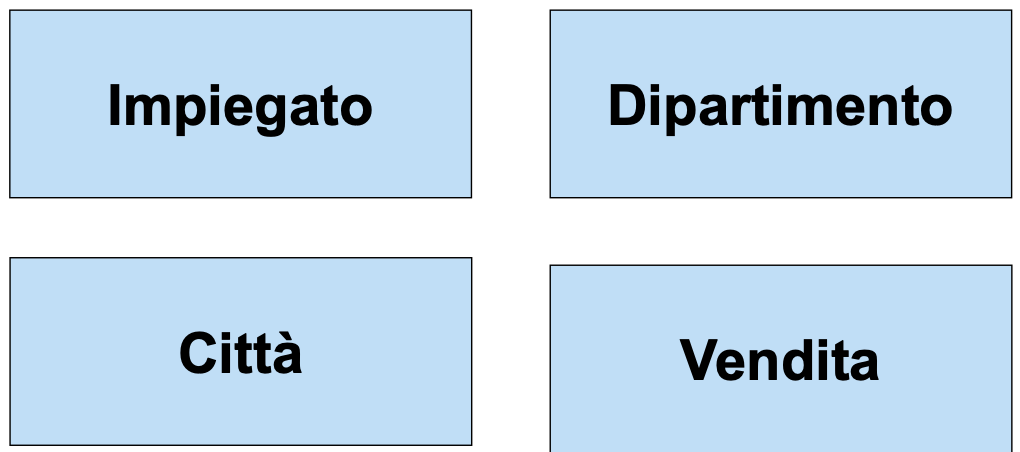
\includegraphics[width=0.5\linewidth]{../images/entita.png}
    \caption{entita}
    %\label{label}
\end{figure}
Nel diagramma ER, ogni entità:
\begin{itemize}
    \item È rappresentata graficamente da un \textbf{rettangolo} contenente il nome dell'entità.
    \item Possiede un \textbf{nome univoco} all'interno dello schema, quindi due entità differenti non possono avere lo stesso nome.
\end{itemize}
\noindent Ad esempio, le entità \texttt{Impiegato} e \texttt{Dipartimento} vengono rappresentate mediante due rettangoli distinti con i rispettivi nomi al loro interno.

\subsubsection{Semantica delle entità}

A livello \textbf{estensionale}, un'entità è rappresentata dal \textbf{un insieme di oggetti}, che sono chiamati le sue \textbf{istanze} o \textbf{occorrenze}.\\
Formalmente, dato:
\begin{itemize}
    \item $S$: uno schema concettuale.
    \item $I$: un'istanza dello schema $S$.
    \item $E$: un'entità definita nello schema $S$.
\end{itemize}
\noindent L'insieme delle istanze dell'entità $E$ nell'istanza $I$ è indicato con:
\[
\operatorname{istanze}(I,E) = \{e_1,e_2,e_3,\ldots\}
\]
Tale insieme prende il nome di \textbf{estensione dell'entità $E$}.\\
\textcolor{verdeEsempio}{Esempio}: se $E = \texttt{Studente}$, la sua estensione contiene tutti gli studenti presenti nella base di dati in quel momento.\\
\textbf{Osservazione importante}: un'istanza di entità rappresenta \textbf{l'oggetto stesso}, non il valore di una sua proprietà. Ad esempio, uno specifico studente è un'istanza dell'entità \texttt{Studente}, mentre il suo nome o la sua matricola sono valori di attributi.\\
Per identificare un oggetto si può utilizzare un \textbf{identificatore univoco} (\textit{object identifier}), che lo distingue dagli altri oggetti.

\subsection*{Entità e istanze di entità}

Nel modello ER è importante distinguere tra \textbf{entità} e \textbf{istanza di entità}:
\begin{itemize}
    \item \textbf{Entità}: rappresenta, nello schema concettuale $S$, una classe di oggetti simili, caratterizzati da proprietà comuni.
    \item \textbf{Istanza di entità}: rappresenta un singolo oggetto appartenente alla classe definita dall'entità, in una determinata istanza dello schema.
\end{itemize}
\noindent \textcolor{verdeEsempio}{Esempio}: \texttt{Studente} è un'entità, mentre uno specifico studente, come Mario Rossi, è una sua istanza.\\
\textbf{Osservazione}: nello schema concettuale vengono rappresentate le \textbf{entità}, non le singole istanze. Questo principio prende il nome di \textbf{astrazione}, perché si descrivono le caratteristiche comuni degli oggetti senza elencarli singolarmente.

\subsection{Attributi di entità}

Un \textbf{attributo di entità} rappresenta una \textbf{proprietà locale} degli oggetti appartenenti a un'entità.\\
Ogni attributo associa a ciascuna istanza dell'entità un valore appartenente a un insieme di valori ammissibili, chiamato \textbf{dominio}.\\
Ad esempio, per l'entità \texttt{Impiegato} possiamo definire:
\begin{itemize}
    \item \textbf{Cognome}: dominio delle stringhe.
    \item \textbf{Età}: dominio degli interi.
    \item \textbf{Stipendio}: dominio dei valori numerici.
\end{itemize}
\noindent Una proprietà è detta \textbf{locale} quando il suo valore dipende esclusivamente dall'oggetto stesso e non dalle relazioni con altri oggetti.\\
Ad esempio, il cognome di un impiegato è una proprietà locale, mentre il dipartimento in cui lavora coinvolge anche un'altra entità e può essere rappresentato tramite una relazione.

\subsubsection{Sintassi: rappresentazione grafica degli attributi}

Nel diagramma ER:
\begin{itemize}
    \item Ogni attributo è rappresentato da un \textbf{cerchio} collegato mediante una linea all'entità.
    \item Il nome dell'attributo viene scritto vicino al cerchio.
    \item Gli attributi della stessa entità devono avere \textbf{nomi distinti}.
\end{itemize}
\noindent \textcolor{verdeEsempio}{Esempio}: rappresentazione dell'entità \texttt{Impiegato} con i suoi attributi.

\begin{center}
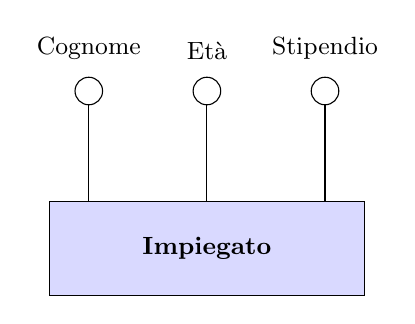
\begin{tikzpicture}[scale=1, every node/.style={font=\small}]
    % Entità
    \node[draw, rectangle, minimum width=4cm,
          minimum height=1.2cm, fill=blue!15]
          (imp) at (0,0) {\textbf{Impiegato}};

    % Attributi
    \node[draw, circle, minimum size=0.35cm,
          inner sep=0pt] (c) at (-1.5,2) {};
    \node[draw, circle, minimum size=0.35cm,
          inner sep=0pt] (e) at (0,2) {};
    \node[draw, circle, minimum size=0.35cm,
          inner sep=0pt] (s) at (1.5,2) {};

    % Collegamenti
    \draw (c.south) -- (-1.5,0.6);
    \draw (e.south) -- (0,0.6);
    \draw (s.south) -- (1.5,0.6);

    % Nomi attributi
    \node[above=0.1cm] at (c.north) {Cognome};
    \node[above=0.1cm] at (e.north) {Età};
    \node[above=0.1cm] at (s.north) {Stipendio};
\end{tikzpicture}
\end{center}

\subsubsection{Dominio di un attributo}

Il \textbf{dominio} è l'insieme dei valori che un attributo può assumere.\\
Generalmente, nel diagramma ER il dominio \textbf{non viene indicato graficamente}, ma viene specificato nel \textbf{dizionario dei dati}, un documento che descrive le caratteristiche degli elementi dello schema.\\
Se si vuole indicare il dominio direttamente nel diagramma, si utilizza la notazione:
\[
\texttt{NomeAttributo/Dominio}
\]
Ad esempio:
\begin{itemize}
    \item \texttt{Cognome/stringa}: il cognome assume valori di tipo stringa.
    \item \texttt{Stipendio/intero}: lo stipendio assume valori interi.
\end{itemize}

\subsubsection{Semantica degli attributi di entità}

A livello \textbf{estensionale}, un attributo associa a ogni istanza di un'entità \textbf{uno e un solo valore} appartenente al suo dominio.\\
Formalmente, considerando:
\begin{itemize}
    \item $S$: uno schema concettuale.
    \item $I$: un'istanza dello schema $S$.
    \item $E$: un'entità dello schema.
    \item $A$: un attributo dell'entità $E$.
    \item $D$: il dominio dell'attributo $A$.
\end{itemize}
\noindent L'attributo $A$ è una \textbf{funzione totale}:
\[
A : \operatorname{istanze}(I,E) \longrightarrow D
\]
Questo significa che:
\begin{itemize}
    \item \textbf{Totale}: ogni istanza dell'entità deve avere un valore associato all'attributo.
    \item \textbf{Univoca}: a ogni istanza viene associato esattamente un valore dell'attributo.
\end{itemize}
\noindent Dal punto di vista matematico, l'attributo può essere rappresentato come un insieme di coppie $(x,y)$, dove $x$ è un'istanza dell'entità e $y$ è il valore dell'attributo associato.\medskip\\
\textcolor{verdeEsempio}{Esempio}: considerando l'attributo \texttt{Età} dell'entità \texttt{Impiegato}:
\[
\operatorname{istanze}(I,\texttt{Età}) =
\{(e_1,25),(e_2,30),(e_3,42)\}
\]
Ogni impiegato è associato a un unico valore di età.
\subsubsection{Esercizi sulle istanze degli attributi}

Consideriamo uno schema ER contenente l'entità \texttt{Impiegato} e l'attributo \texttt{Età}, il cui dominio è l'insieme dei numeri interi.\\
L'attributo \texttt{Età} deve essere una \textbf{funzione totale}:
\[
\text{Età}: \operatorname{istanze}(I,\texttt{Impiegato})
\longrightarrow \mathbb{Z}
\]
Questo significa che \textbf{ogni impiegato deve avere esattamente un valore di età}.\\
Vediamo tre casi per capire quando un insieme di dati rappresenta un'istanza valida dello schema.

\subsubsection{Esercizio 1: istanza valida}

Consideriamo quattro impiegati e le seguenti associazioni:
\begin{figure}[H]
    \centering  
    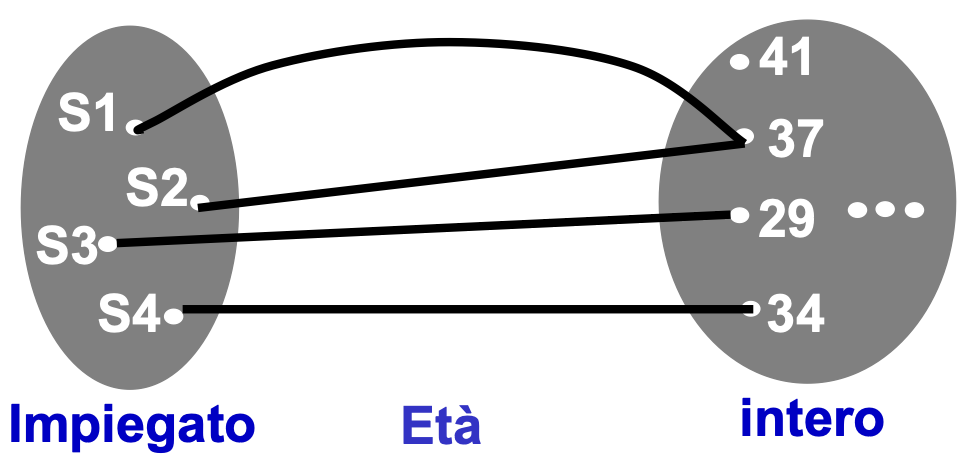
\includegraphics[width=0.4\linewidth]{../images/attributi_1.png}
    %\caption{caption}
    %\label{label}
\end{figure}
\noindent \textbf{Risposta: SÌ, è un'istanza valida.}\\
Ogni impiegato possiede uno e un solo valore di età.\\
\textbf{Osservazione}: due impiegati diversi possono avere la stessa età (come $S_1$ e $S_2$). Infatti, un attributo deve essere una funzione totale, ma \textbf{non necessariamente iniettiva}.

\subsubsection{Esercizio 2a: più valori per la stessa istanza}

Consideriamo le associazioni:
\begin{figure}[H]
    \centering  
    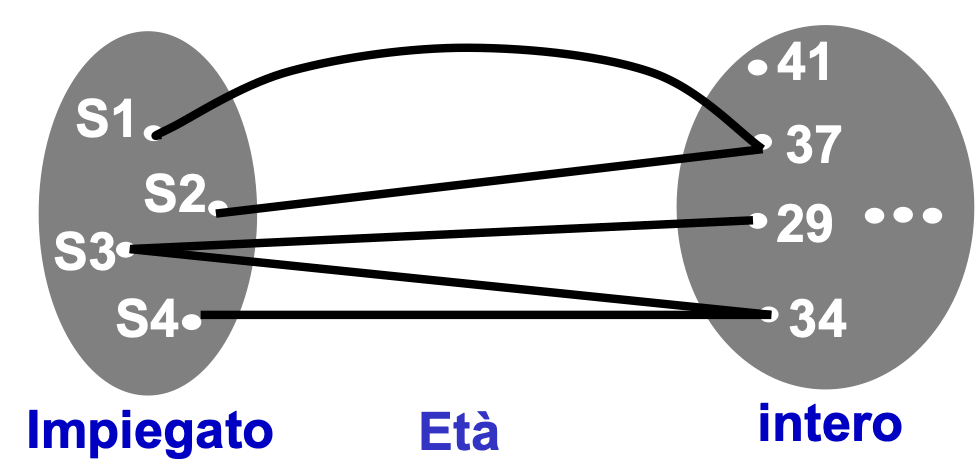
\includegraphics[width=0.4\linewidth]{../images/attributi_2.png}
    %\caption{caption}
    %\label{label}
\end{figure}
\noindent \textbf{Risposta: NO, non è un'istanza valida.}\\
L'impiegato $S_3$ è associato a \textbf{due valori differenti} dell'attributo \texttt{Età}.\\
Questo viola la definizione di funzione, perché \textbf{a ogni elemento del dominio deve corrispondere un unico valore}.

\subsubsection{Esercizio 2b: valore mancante}

Consideriamo le associazioni:
\begin{figure}[H]
    \centering  
    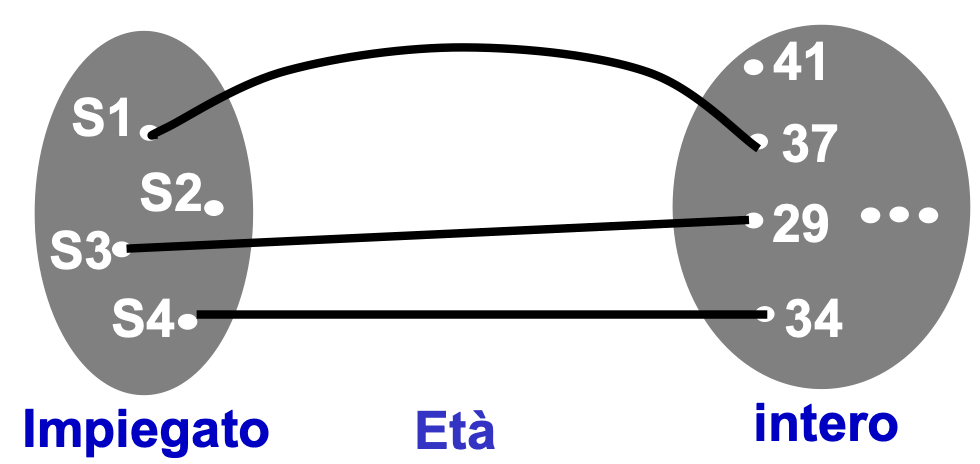
\includegraphics[width=0.4\linewidth]{../images/attributi_3.png}
    %\caption{caption}
    %\label{label}
\end{figure}
\noindent \textbf{Risposta: NO, non è un'istanza valida.}\\
L'impiegato $S_2$ non possiede alcun valore associato all'attributo \texttt{Età}.\\
Questo viola la proprietà di \textbf{totalità}, secondo cui ogni istanza dell'entità deve avere un valore dell'attributo.

\subsection{Relazioni}

Nel modello Entità-Relazione (ER), una \textbf{relazione}
(o associazione) rappresenta un \textbf{legame logico}
tra due o più entità.
Il numero di entità coinvolte, più precisamente
il numero di ruoli o partecipazioni, determina
il \textbf{grado della relazione}:
\begin{itemize}
    \item \textbf{Relazione binaria}: coinvolge due
    partecipazioni di entità (grado 2).
    \item \textbf{Relazione ternaria}: coinvolge tre
    partecipazioni (grado 3).
    \item \textbf{Relazione n-aria}: coinvolge
    $n$ partecipazioni (grado $n$).
\end{itemize}
\noindent
\textbf{Esempi:}
\begin{itemize}
    \item \textit{Residenza}: collega Persona e Città.
    \item \textit{Afferenza}: collega Impiegato e Dipartimento.
    \item \textit{EsameSuperato}: collega Studente e Corso.
\end{itemize}
\noindent
Una relazione non descrive le caratteristiche
di una singola entità, ma il legame esistente
tra le entità coinvolte.

\subsubsection{Rappresentazione grafica delle relazioni}

Nel diagramma ER, una relazione è rappresentata
attraverso un \textbf{rombo}, contenente il nome
della relazione e collegato alle entità partecipanti.\\
Ogni relazione possiede un nome che la identifica
univocamente all'interno dello schema.\\
Ad esempio, consideriamo:
\begin{itemize}
    \item \textbf{Studente}, con attributi Cognome ed Età.
    \item \textbf{Corso}, con attributi Nome e Crediti.
    \item \textbf{EsameSuperato}, relazione che collega
    Studente e Corso.
\end{itemize}
\begin{figure}[H]
    \centering  
    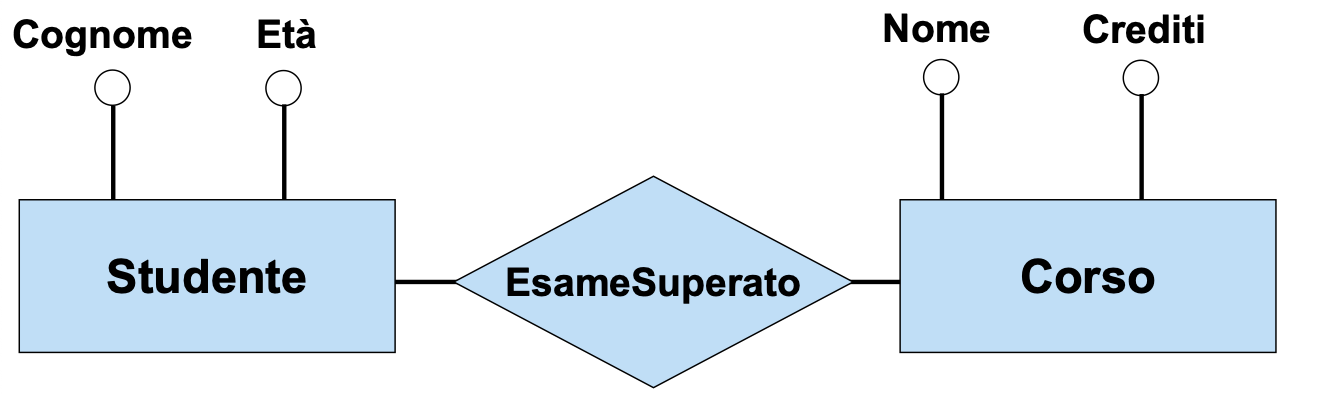
\includegraphics[width=0.4\linewidth]{../images/rel1.png}
    %\caption{caption}
    %\label{label}
\end{figure}

\subsubsection{Semantica delle relazioni binarie}

Per comprendere il significato di una relazione
distinguiamo:
\begin{itemize}
    \item \textbf{Livello intensionale}: descrive
    la struttura della relazione, cioè quali
    entità collega.
    \item \textbf{Livello estensionale}: descrive
    le effettive associazioni tra le istanze
    delle entità in un determinato momento.
\end{itemize}
\noindent
Consideriamo una relazione binaria $R$
tra le entità $E$ ed $F$.\\
A livello estensionale, ogni \textbf{istanza
della relazione} è una coppia etichettata:
\[
(E:x,\;F:y)
\]
dove:
\begin{itemize}
    \item $x$ è un'istanza dell'entità $E$;
    \item $y$ è un'istanza dell'entità $F$.
\end{itemize}
\noindent
Le etichette $E$ ed $F$ specificano
il ruolo delle due componenti nella relazione.\\
L'insieme di tutte le coppie che partecipano
alla relazione costituisce la sua
\textbf{estensione}.

\subsubsection{Definizione matematica}

Sia $S$ uno schema ER e $I$ una sua istanza.\\
Indichiamo con:
\begin{itemize}
    \item $\operatorname{istanze}(I,E)$:
    l'insieme delle istanze dell'entità $E$;
    \item $\operatorname{istanze}(I,F)$:
    l'insieme delle istanze dell'entità $F$;
    \item $\operatorname{istanze}(I,R)$:
    l'insieme delle istanze della relazione $R$.
\end{itemize}
\noindent
Una relazione binaria è, dal punto di vista
matematico, un sottoinsieme del prodotto
cartesiano delle istanze delle entità:
\[
\boxed{
\operatorname{istanze}(I,R)
\subseteq
\operatorname{istanze}(I,E)
\times
\operatorname{istanze}(I,F)
}
\]
Le coppie sono considerate etichettate
in base alle entità partecipanti.\\
\textbf{Significato:} il prodotto cartesiano
contiene tutte le possibili coppie tra
le istanze di $E$ ed $F$, mentre la relazione
contiene soltanto quelle per cui
il legame esiste effettivamente.\medskip\\
\textbf{Esempio: EsameSuperato}\\
Supponiamo di avere:
\[
Studente=\{S1,S2,S3,S4\}
\]
\[
Corso=\{C1,C2,C3,C4\}
\]
L'estensione della relazione potrebbe essere:
\[
\begin{aligned}
EsameSuperato=\{&
(S1,C1),\\
&(S2,C2),\\
&(S2,C3),\\
&(S3,C3)\}
\end{aligned}
\]
Questo significa che:
\begin{itemize}
    \item $S1$ ha superato l'esame $C1$;
    \item $S2$ ha superato gli esami $C2$ e $C3$;
    \item $S3$ ha superato l'esame $C3$;
    \item $S4$ non compare nella relazione,
    perché non risulta aver superato alcun esame.
\end{itemize}
\begin{figure}[H]
    \centering  
    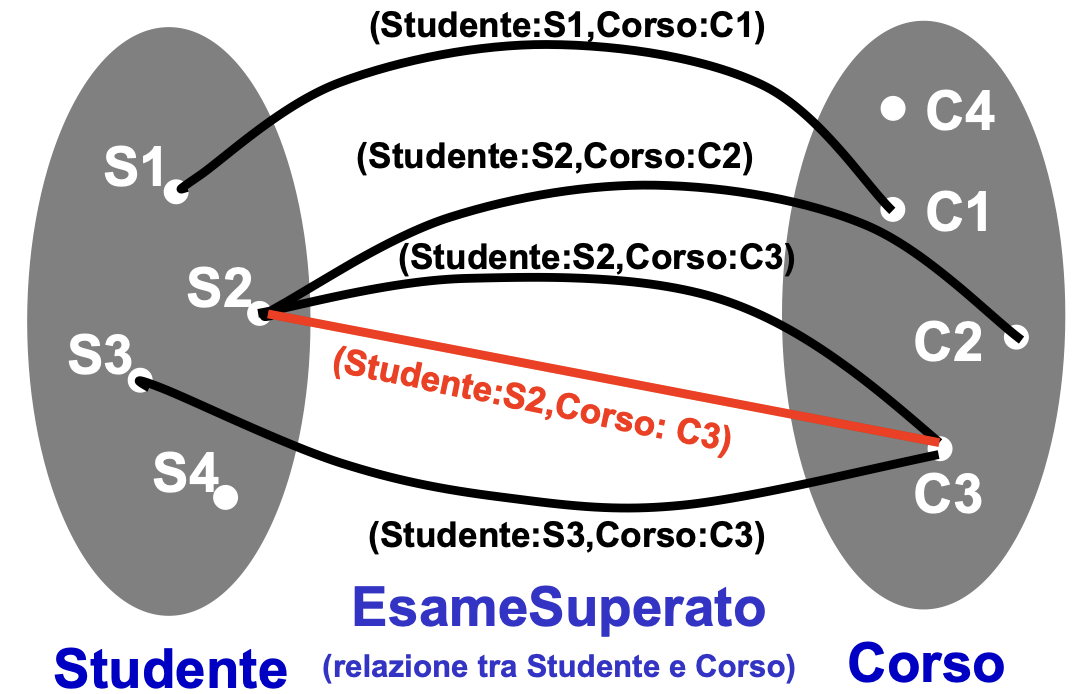
\includegraphics[width=0.4\linewidth]{../images/rel2.png}
    %\caption{caption}
    %\label{label}
\end{figure}
\noindent
\textbf{Osservazione fondamentale:}\\
Una stessa istanza di entità può partecipare
a più istanze della relazione, purché
le coppie siano diverse.\\
Ad esempio, lo studente $S2$ può essere
associato sia a $C2$ sia a $C3$.

\subsubsection{Unicità delle istanze di relazione}

Una proprietà fondamentale del modello ER è che
\textbf{non possono esistere due istanze distinte
della stessa relazione che coinvolgano
esattamente le stesse istanze di entità},
negli stessi ruoli.\\
Infatti, una relazione è matematicamente
un \textbf{insieme di tuple}, e negli insiemi
non sono ammesse ripetizioni.

\subsection*{Relazioni n-arie}

Una \textbf{relazione n-aria} è una relazione
che coinvolge $n$ partecipazioni di entità.\\
Quando il grado è maggiore di 2, si parla
di relazione n-aria non binaria.\\
Un esempio è la relazione ternaria
\textbf{Fornitura}, che coinvolge:
\begin{itemize}
    \item \textbf{Fornitore}: chi fornisce il prodotto;
    \item \textbf{Dipartimento}: chi riceve il prodotto;
    \item \textbf{Prodotto}: il bene fornito.
\end{itemize}
\begin{figure}[H]
    \centering  
    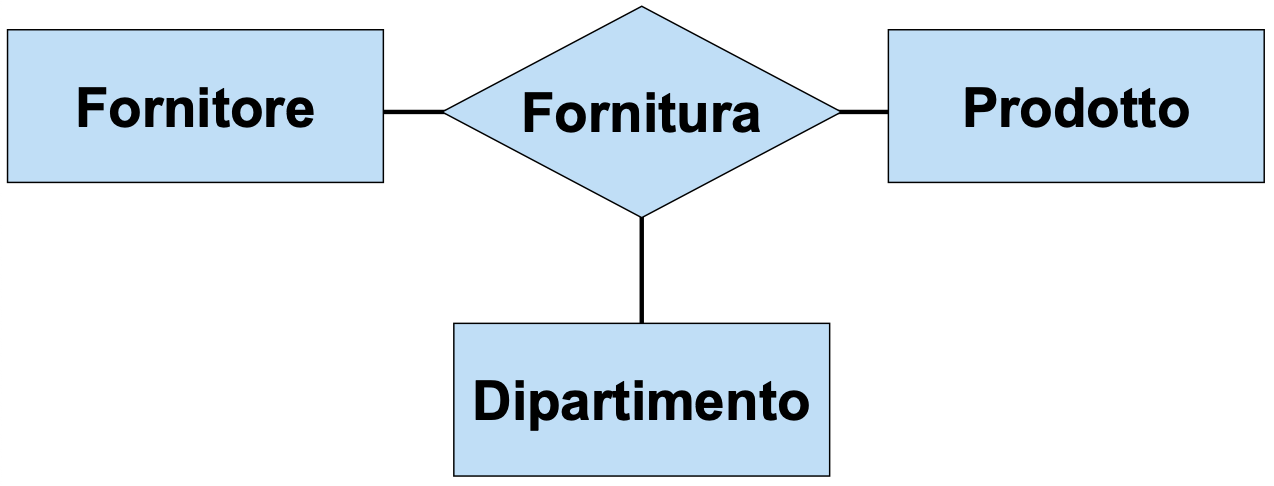
\includegraphics[width=0.4\linewidth]{../images/rel3.png}
    %\caption{caption}
    %\label{label}
\end{figure}
\noindent
Ogni istanza della relazione rappresenta
una specifica fornitura effettuata da
un fornitore, verso un dipartimento,
per un determinato prodotto.\\
Essendo coinvolte tre entità,
la relazione ha \textbf{grado 3}.

\subsubsection{Semantica delle relazioni n-arie}

Consideriamo una relazione $R$ definita
sulle entità $E_1,E_2,\ldots,E_n$,
inizialmente supposte distinte.\\
Ogni istanza della relazione è una
\textbf{n-pla etichettata}:
\[
(E_1:x_1,\;E_2:x_2,\;\ldots,\;E_n:x_n)
\]
dove ogni $x_i$ è un'istanza
dell'entità $E_i$.\\
L'estensione della relazione è quindi
un sottoinsieme del prodotto cartesiano:
\[
\boxed{
\operatorname{istanze}(I,R)
\subseteq
\prod_{i=1}^{n}
\operatorname{istanze}(I,E_i)
}
\]
Ovvero:
\[
\operatorname{istanze}(I,R)
\subseteq
\operatorname{istanze}(I,E_1)
\times\cdots\times
\operatorname{istanze}(I,E_n)
\]
Anche in questo caso le tuple
sono etichettate e non possono
comparire duplicati.\medskip\\
\textbf{Esempio: Fornitura}\\
Supponiamo che l'estensione della relazione
sia composta dalle seguenti triple:
\[
\begin{aligned}
Fornitura=\{&
(F1,D1,P1),\\
&(F3,D2,P3),\\
&(F3,D4,P3)\}
\end{aligned}
\]
Queste triple rappresentano tre forniture:
\begin{itemize}
    \item $F1$ fornisce $P1$ al dipartimento $D1$;
    \item $F3$ fornisce $P3$ al dipartimento $D2$;
    \item $F3$ fornisce $P3$ al dipartimento $D4$.
\end{itemize}
\noindent
Le ultime due triple sono distinte,
anche se coinvolgono lo stesso fornitore
e lo stesso prodotto, perché il dipartimento
è diverso.\\
Non sarebbe invece possibile inserire
due volte la tripla $(F3,D2,P3)$
come due istanze distinte della relazione.

\begin{figure}[H]
    \centering  
    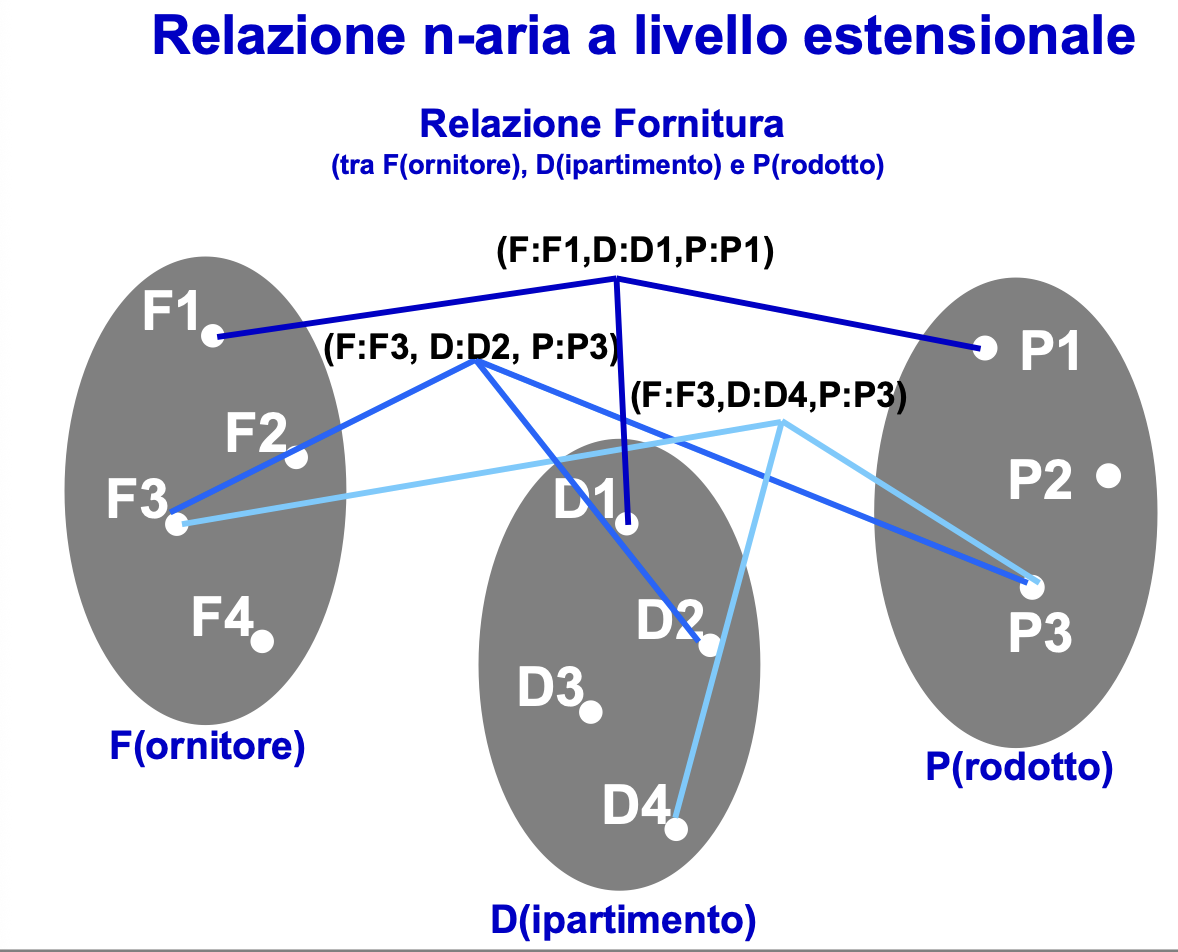
\includegraphics[width=0.5\linewidth]{../images/rel4.png}
    %\caption{caption}
    %\label{label}
\end{figure}

\subsection*{Più relazioni tra le stesse entità}

Le stesse entità possono essere coinvolte
in \textbf{più relazioni differenti},
purché ciascuna rappresenti
un legame con un significato diverso.\\
Ad esempio, consideriamo le entità:
\begin{itemize}
    \item \textbf{Impiegato};
    \item \textbf{Città}.
\end{itemize}
\noindent
Tra queste entità possiamo definire:
\begin{itemize}
    \item \textbf{Residenza}: indica la città
    in cui risiede l'impiegato;
    \item \textbf{SedeDiLavoro}: indica la città
    in cui l'impiegato lavora.
\end{itemize}
\noindent
Le due relazioni sono indipendenti,
anche se collegano le stesse entità.\\
Ad esempio, un impiegato può risiedere
a Roma ma lavorare a Milano.
\begin{figure}[H]
    \centering  
    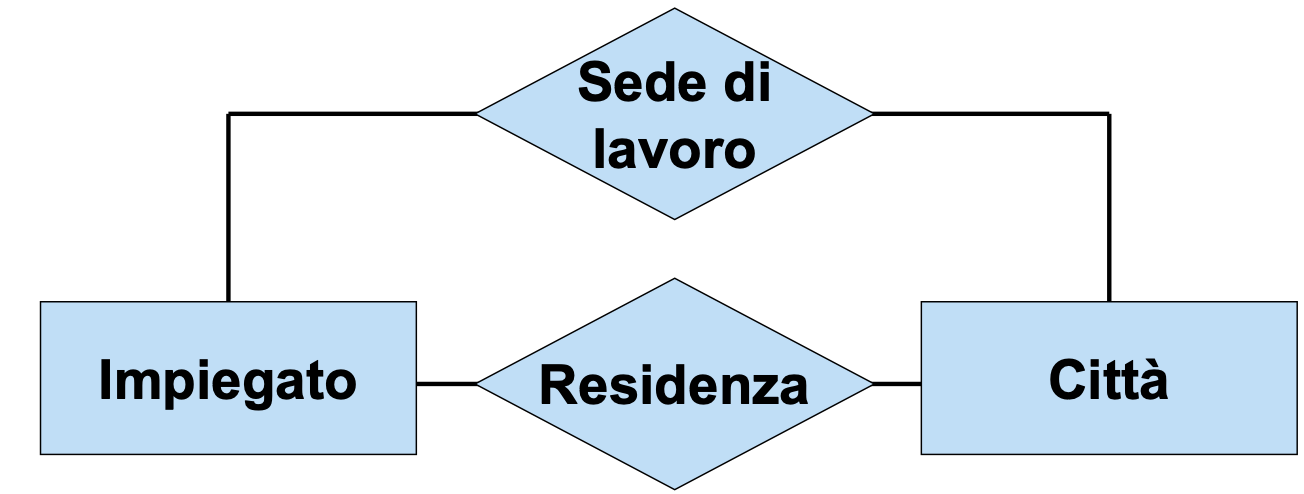
\includegraphics[width=0.4\linewidth]{../images/rel5.png}
    %\caption{caption}
    %\label{label}
\end{figure}

\subsection*{Attributi di relazione}

Un \textbf{attributo di relazione} rappresenta
una proprietà del \textbf{legame tra le entità},
e non una proprietà delle singole entità.\\
Analogamente agli attributi delle entità,
ogni attributo di relazione:
\begin{itemize}
    \item Ha un nome univoco nell'ambito
    della relazione;
    \item Possiede un dominio, cioè
    un insieme di valori ammissibili;
    \item Associa un valore a ogni istanza
    della relazione.
\end{itemize}
\noindent
Nel diagramma ER, un attributo di relazione
viene rappresentato con un \textbf{cerchio}
collegato direttamente al rombo
della relazione.

\subsubsection{Esempio: attributo Voto}

Consideriamo la relazione:
\[
EsameSuperato(Studente,Corso)
\]
Possiamo aggiungere l'attributo
\textbf{Voto}, che indica il voto
ottenuto da uno studente in un corso.\\
Il voto non è una proprietà dello studente,
perché uno studente può ottenere
voti diversi in corsi diversi.\\
Non è nemmeno una proprietà del corso,
perché studenti diversi possono ottenere
voti diversi nello stesso corso.\\
È quindi una proprietà del
\textbf{legame Studente-Corso}.\medskip\\
\textbf{Esempio concreto:}
\[
\begin{aligned}
(S2,C2)&\longrightarrow 25\\
(S2,C3)&\longrightarrow 19\\
(S3,C3)&\longrightarrow 25
\end{aligned}
\]
\begin{figure}[H]
    \centering  
    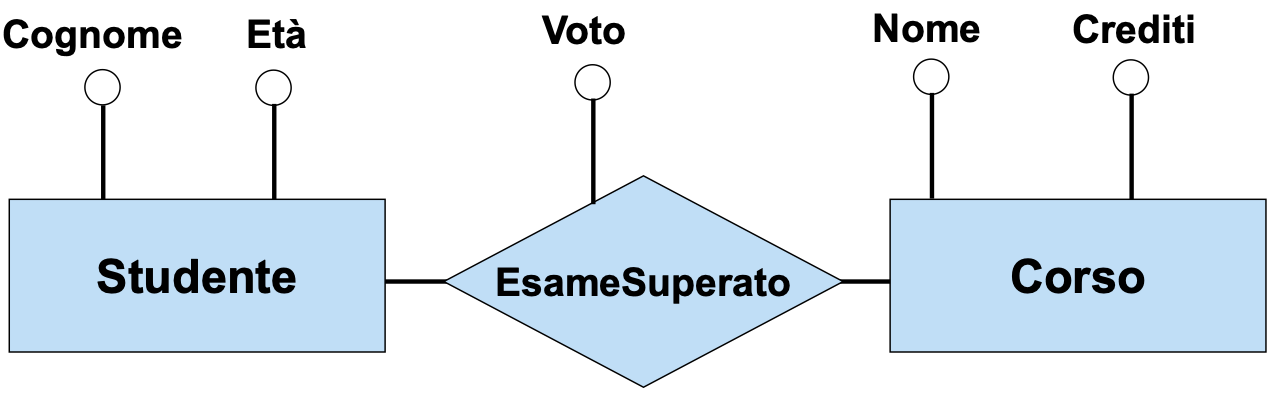
\includegraphics[width=0.4\linewidth]{../images/rel6.png}
    %\caption{caption}
    %\label{label}
\end{figure}

\subsection*{Semantica degli attributi di relazione}

Dal punto di vista matematico,
un attributo di relazione è una
\textbf{funzione totale}.\\
Sia:
\begin{itemize}
    \item $S$ uno schema ER;
    \item $I$ un'istanza dello schema;
    \item $R$ una relazione;
    \item $A$ un attributo di $R$;
    \item $D$ il dominio dell'attributo $A$.
\end{itemize}
\noindent
Allora l'attributo $A$ è definito come:
\[
\boxed{
A:\operatorname{istanze}(I,R)\rightarrow D
}
\]
Questo significa che \textbf{a ogni istanza
della relazione viene associato
uno e un solo valore del dominio}.\\
\textbf{Osservazione fondamentale:}\\
Gli attributi di relazione
\textbf{non distinguono istanze diverse
della stessa relazione}.\\
Infatti, l'identità di un'istanza
dipende esclusivamente dalle istanze
di entità coinvolte nel legame.\\
Quindi, anche se due voti sono diversi,
non possiamo rappresentare due istanze
distinte di \textit{EsameSuperato}
che coinvolgono lo stesso studente
e lo stesso corso.\\
Per rappresentare più eventi distinti
servirebbe modificare il modello concettuale.

\subsection*{Attributi di relazioni n-arie}

Anche una relazione n-aria può possedere
attributi che descrivono proprietà
del legame tra tutte le entità coinvolte.\\
Consideriamo la relazione ternaria:
\[
Fornitura(Fornitore,Dipartimento,Prodotto)
\]
Possiamo introdurre l'attributo
\textbf{Quantità}, che rappresenta
la quantità di prodotto fornita
da un determinato fornitore
a un determinato dipartimento.\\
La quantità non dipende soltanto
dal fornitore, dal dipartimento
o dal prodotto considerati singolarmente,
ma dalla \textbf{specifica tripla}
che costituisce la fornitura.
\begin{figure}[H]
    \centering  
    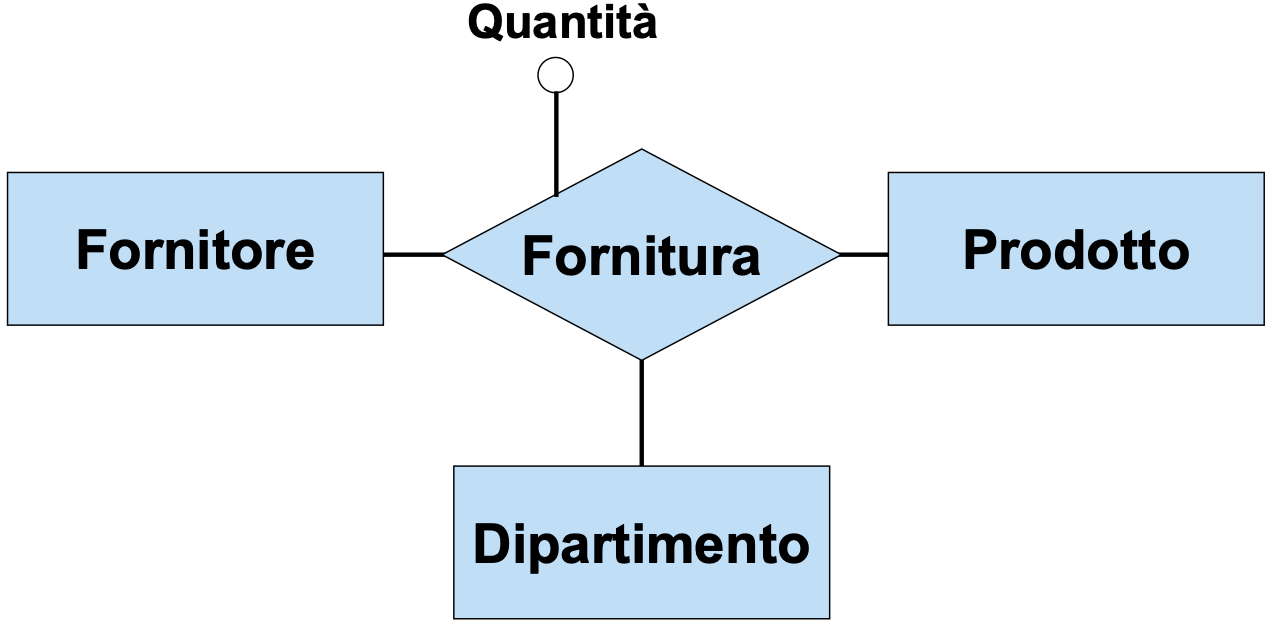
\includegraphics[width=0.4\linewidth]{../images/rel7.png}
    %\caption{caption}
    %\label{label}
\end{figure}
\noindent \textbf{Esempio:}
\[
\begin{aligned}
(F1,D1,P1)&\longrightarrow 89\\
\end{aligned}
\]
Ogni tripla rappresenta una diversa
istanza della relazione \textit{Fornitura},
alla quale viene associata una quantità.\\
Formalmente:
\[
Quantita:
\operatorname{istanze}(I,Fornitura)
\rightarrow \mathbb{N}
\]
dove $\mathbb{N}$ rappresenta
il dominio dei numeri naturali,
assumendo che le quantità siano intere
e non negative.
\subsubsection{Esercizio}
Descrivere lo schema concettuale della seguente realtà:\\
I docenti hanno un codice fiscale ed una età. I docenti
operano nei corsi di laurea (si dice che afferiscono ai
corsi di laurea). Interessa la data di afferenza dei
docenti ai corsi di laurea. I corsi di laurea hanno un
codice ed un nome, ed appartengono alle facoltà.
Ogni facoltà ha un nome.\\
\underline{soluzione}:\\
\begin{figure}[H]
      
    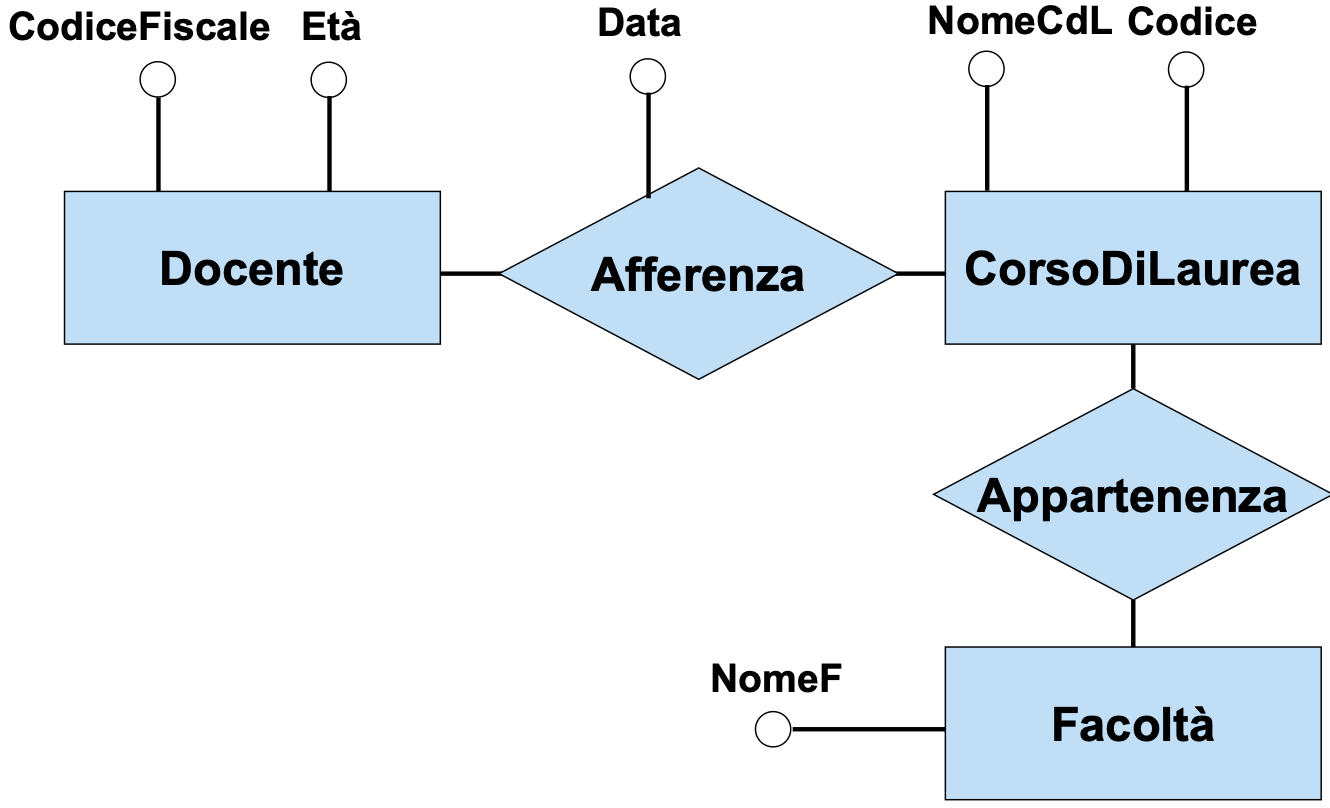
\includegraphics[width=0.5\linewidth]{../images/rel8.png}
    %\caption{caption}
    %\label{label}
\end{figure}

\subsection*{Relazioni sulla stessa entità}
Una relazione può coinvolgere \textbf{la stessa entità più volte}.
In questo caso è necessario distinguere il significato di ciascuna
partecipazione attraverso i \textbf{ruoli}.
\begin{figure}[H]
    \centering
    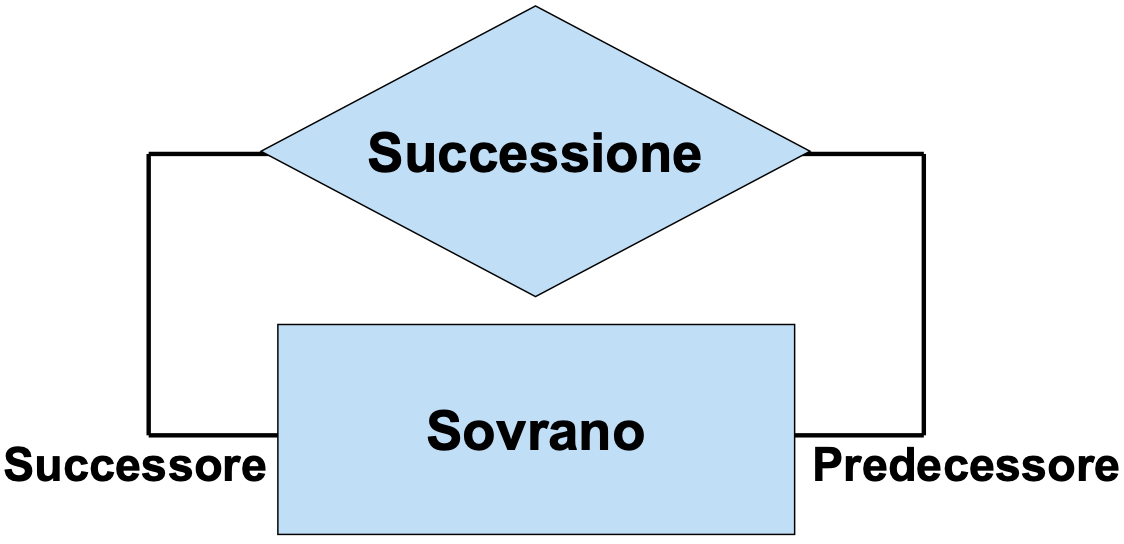
\includegraphics[width=0.4\linewidth]{../images/rel9.png}
    %\caption{caption}
    %\label{label}
\end{figure}
\noindent
L'entità Sovrano partecipa due volte alla relazione Successione,
ma con ruoli differenti:
\begin{itemize}
    \item \textbf{Predecessore}: il sovrano che viene prima;
    \item \textbf{Successore}: il sovrano che viene dopo.
\end{itemize}

\noindent
Senza i ruoli non sarebbe possibile distinguere chi precede
e chi succede all'interno della relazione.

\subsubsection*{Definizione di ruolo}

Un \textbf{ruolo} specifica la funzione che un'entità svolge
all'interno di una relazione.\\
Se un'entità $E$ partecipa a una relazione $R$ con ruolo $U$,
significa che ogni sua partecipazione a $R$ viene identificata
attraverso il ruolo $U$.

\subsubsection*{Rappresentazione grafica dei ruoli}

Nel diagramma Entità-Relazione:
\begin{itemize}
    \item il nome del ruolo viene scritto vicino al collegamento
    tra l'entità e la relazione;
    \item ogni partecipazione a una relazione deve avere un ruolo,
    anche quando le entità coinvolte sono differenti;
    \item se il nome del ruolo non viene specificato, si assume
    che coincida con il nome dell'entità;
    \item due collegamenti della stessa relazione non possono
    avere lo stesso nome di ruolo.
\end{itemize}

\noindent
\textbf{Importante:} i ruoli sono particolarmente necessari
nelle relazioni ricorsive, cioè quelle in cui una stessa entità
partecipa più volte alla medesima relazione.

\subsection*{Semantica dei ruoli e delle relazioni}

L'introduzione dei ruoli modifica il modo in cui rappresentiamo
le istanze delle relazioni.
In precedenza, le tuple erano etichettate con i nomi delle entità.
Ora, invece, vengono etichettate con i \textbf{nomi dei ruoli}.\\
Consideriamo una relazione $R$ tra le entità
$E_1,E_2,\ldots,E_n$, con rispettivi ruoli
$U_1,U_2,\ldots,U_n$.\\
Le entità coinvolte non devono necessariamente essere tutte
differenti, mentre i nomi dei ruoli devono essere distinti.
In una determinata istanza $I$ dello schema $S$,
ogni istanza della relazione $R$ è una tupla etichettata
della forma:

\[
(U_1:x_1,\ U_2:x_2,\ \ldots,\ U_n:x_n)
\]
dove:
\begin{itemize}
    \item $U_i$ rappresenta il ruolo;
    \item $x_i$ rappresenta un'istanza dell'entità $E_i$;
    \item $x_i \in istanze(I,E_i)$.
\end{itemize}
\noindent
L'insieme di tutte queste tuple costituisce
l'\textbf{estensione della relazione} $R$ nell'istanza $I$,
indicata con:

\[
istanze(I,R)
\]

\subsubsection*{Esempio: Successione tra sovrani}

Consideriamo l'entità:

\[
Sovrano
\]

e la relazione:

\[
Successione
\]

con i due ruoli:
\begin{itemize}
    \item \textbf{Predecessore};
    \item \textbf{Successore}.
\end{itemize}

\noindent
Supponiamo che nell'istanza $I$ siano presenti i sovrani:
\[
istanze(I,Sovrano)=
\{romolo,numa,tullo,anco\}
\]
L'estensione della relazione Successione è:

\[
\begin{aligned}
istanze(I,Successione)=\{&
(Predecessore:romolo,\ Successore:numa),\\
&(Predecessore:numa,\ Successore:tullo),\\
&(Predecessore:tullo,\ Successore:anco)
\}
\end{aligned}
\]

\noindent
\textbf{Osservazione importante:} ogni tupla contiene
due istanze dell'entità Sovrano, ma i ruoli permettono
di distinguere il predecessore dal successore.



% ============================================================
% SCELTA TRA ENTITÀ E RELAZIONE
% ============================================================

\subsection{Scelta tra entità e relazione}

Durante la progettazione concettuale è necessario stabilire
se un determinato concetto debba essere rappresentato
mediante un'\textbf{entità} oppure mediante una
\textbf{relazione}.\\
La scelta dipende principalmente dal significato che
il concetto assume nel contesto applicativo.

\subsubsection*{Quando utilizzare un'entità}

Un concetto dovrebbe essere modellato come
\textbf{entità} quando:

\begin{itemize}
    \item Le sue istanze hanno un significato autonomo,
    indipendentemente dall'esistenza di altre istanze.

    \item Possiede, oppure potrebbe possedere,
    attributi propri.

    \item Può partecipare a relazioni con altri concetti.
\end{itemize}
\noindent
\textcolor{verdeEsempio}{\textbf{Esempio.}}
Il concetto di \textit{Persona} deve essere rappresentato
come entità, perché ogni persona esiste indipendentemente
dalle sue proprietà, come cognome, età e città di nascita.

\subsubsection*{Quando utilizzare una relazione}

Un concetto dovrebbe essere modellato come
\textbf{relazione} quando:

\begin{itemize}
    \item Le sue istanze non hanno significato autonomo,
    ma rappresentano associazioni tra istanze
    di altre entità.

    \item Non ha senso considerare le sue istanze
    come oggetti che partecipano autonomamente
    ad altre relazioni.
\end{itemize}
\noindent
\textcolor{verdeEsempio}{\textbf{Esempio.}}
Il concetto di \textit{Frequenta}, che associa
uno studente a un corso, può essere rappresentato
come relazione tra le entità \textit{Studente}
e \textit{Corso}.

\subsubsection*{Esercizio 10: scelta tra entità e relazione}

Si consideri uno schema:
\begin{center}
\begin{tikzpicture}

% Relazione Persona (rombo disegnato manualmente)
\draw[thick, fill=lightblue]
    (0,1) -- (1.5,0) -- (0,-1) -- (-1.5,0) -- cycle;

\node at (0,0) {\textbf{Persona}};

% Entità
\node[draw, rectangle, fill=lightblue,
      minimum width=2.8cm, minimum height=1cm]
      (c) at (-4,0) {Cognome};

\node[draw, rectangle, fill=lightblue,
      minimum width=2.8cm, minimum height=1cm]
      (e) at (4,0) {Età};

\node[draw, rectangle, fill=lightblue,
      minimum width=2.8cm, minimum height=1cm]
      (ci) at (0,-3) {Città};

% Collegamenti
\draw[thick] (c.east) -- (-1.5,0);
\draw[thick] (e.west) -- (1.5,0);
\draw[thick] (ci.north) -- (0,-1);

\end{tikzpicture}
\end{center}
\noindent
\textbf{Perché questo schema è sbagliato?}

\begin{enumerate}
    \item \textbf{Persona non è rappresentata
    come entità autonoma.}

    Ogni persona viene identificata attraverso
    una tupla della relazione Persona.

    Questo significa che una persona esiste
    nello schema soltanto in quanto associazione
    tra un cognome, un'età e una città.

    \item \textbf{Cognome ed Età sono modellati
    erroneamente come entità.}

    Nel contesto considerato, cognome ed età
    sono semplicemente proprietà delle persone,
    non oggetti autonomi.

    \item \textbf{Non è possibile distinguere
    persone con le stesse proprietà.}

    Una relazione è un insieme di tuple,
    quindi non può contenere due tuple identiche.

    Di conseguenza, due persone aventi lo stesso
    cognome, la stessa età e la stessa città
    di nascita verrebbero rappresentate
    dalla medesima tupla.
\end{enumerate}
\noindent
\textcolor{verdeEsempio}{\textbf{Soluzione corretta.}}
Il concetto di Persona deve essere modellato
come un'entità, mentre Cognome, Età e Città
di nascita devono essere rappresentati
come attributi.

\begin{center}
\begin{tikzpicture}[
    entity/.style={
        rectangle, draw, fill=lightblue,
        minimum width=3cm,
        minimum height=1.1cm
    },
    attr/.style={
        circle, draw,
        minimum size=0.2cm,
        inner sep=0pt
    }
]

\node[entity] (p) at (0,0) {Persona};

\node[attr] (a1) at (-3,1.8) {};
\node[attr] (a2) at (0,2) {};
\node[attr] (a3) at (3,1.8) {};

\draw (p) -- (a1);
\draw (p) -- (a2);
\draw (p) -- (a3);

\node[above] at (a1) {Cognome};
\node[above] at (a2) {Età};
\node[above, align=center] at (a3) {Città di nascita};

\end{tikzpicture}
\end{center}


% ============================================================
% RELAZIONE ISA
% ============================================================

\subsection{Relazione ISA tra entità}

Nel modello Entità-Relazione può accadere che
due entità abbiano istanze in comune.
Un caso particolarmente importante è quello
in cui tutte le istanze di un'entità appartengono
anche a un'altra entità.\\
Questa situazione viene rappresentata attraverso
la \textbf{relazione ISA}, detta anche
\textbf{relazione di sottoinsieme}.
\subsubsection*{Definizione}

Date due entità $E_1$ ed $E_2$, si dice che

\[
E_1 \text{ ISA } E_2
\]
quando ogni istanza di $E_1$ è anche
un'istanza di $E_2$.\\
In particolare:
\begin{itemize}
    \item $E_1$ è detta \textbf{sottoentità}
    oppure \textbf{entità figlia};

    \item $E_2$ è detta \textbf{entità padre}.
\end{itemize}
\noindent
\textcolor{verdeEsempio}{\textbf{Esempio.}}
Si considerino le entità Persona e Studente.
Ogni studente è una persona, ma non ogni
persona è necessariamente uno studente.
Pertanto:

\[
\text{Studente ISA Persona}
\]

\subsubsection*{Rappresentazione grafica}

La relazione ISA viene rappresentata mediante
una freccia che parte dalla sottoentità
e punta verso l'entità padre.

\begin{center}
\begin{tikzpicture}[
    entity/.style={
        rectangle, draw, fill=lightblue,
        minimum width=3.2cm,
        minimum height=1cm
    }
]

\node[entity] (p) at (0,2.5) {Persona};
\node[entity] (s) at (0,0) {Studente};

\draw[->, thick, >=stealth]
(s.north) -- (p.south);

\end{tikzpicture}
\end{center}

\subsubsection*{Regole della relazione ISA}

Nel modello ER considerato, una sottoentità
può avere \textbf{al massimo un'entità padre}.
Di conseguenza, non è ammessa
l'\textbf{ereditarietà multipla}.
Ad esempio, non è possibile rappresentare
direttamente StudenteLavoratore come sottoentità
sia di Studente sia di Lavoratore.

\subsubsection*{Semantica della relazione ISA}

A livello estensionale, la relazione ISA
impone un vincolo di inclusione tra
gli insiemi delle istanze.
Se
\[
E_1 \text{ ISA } E_2
\]
allora, per ogni istanza $I$ dello schema:
\[
\boxed{
\operatorname{istanze}(I,E_1)
\subseteq
\operatorname{istanze}(I,E_2)
}
\]
Questo significa che tutte le istanze
della sottoentità devono appartenere
anche all'entità padre.\\
\textcolor{verdeEsempio}{\textbf{Esempio.}}
Si considerino:
\[
\operatorname{istanze}(I,\text{Persona})
=
\{a,b,c,d\}
\]
\[
\operatorname{istanze}(I,\text{Studente})
=
\{b,d\}
\]
Questa è un'istanza valida, perché:
\[
\{b,d\}\subseteq\{a,b,c,d\}
\]
Sono valide anche le situazioni in cui:
\[
\operatorname{istanze}(I,\text{Studente})
=
\{a,b,c,d\}
\]
oppure:
\[
\operatorname{istanze}(I,\text{Studente})
=
\varnothing
\]
Non sarebbe invece valida la situazione:
\[
\operatorname{istanze}(I,\text{Persona})
=
\{a\}
\]
\[
\operatorname{istanze}(I,\text{Studente})
=
\{a,b\}
\]
poiché $b$ è uno studente ma non appartiene
all'insieme delle persone.

\subsubsection*{Proprietà della relazione ISA}

La relazione ISA gode di due proprietà
fondamentali.\\
\textbf{1. Riflessività}\\
Ogni entità è in relazione ISA con sé stessa:
\[
E \text{ ISA } E
\]
Infatti:
\[
\operatorname{istanze}(I,E)
\subseteq
\operatorname{istanze}(I,E)
\]
\textbf{2. Transitività}\\
Se:
\[
E_1 \text{ ISA } E_2
\]
e:
\[
E_2 \text{ ISA } E_3
\]
allora:
\[
\boxed{E_1 \text{ ISA } E_3}
\]
\textcolor{verdeEsempio}{\textbf{Esempio.}}
\[
\text{FuoriCorso ISA Studente}
\]
\[
\text{Studente ISA Persona}
\]
Di conseguenza:
\[
\boxed{\text{FuoriCorso ISA Persona}}
\]

% ============================================================
% EREDITARIETÀ
% ============================================================

\subsection{Ereditarietà nel modello ER}

Una conseguenza fondamentale della relazione ISA
è il \textbf{principio di ereditarietà}.
Secondo questo principio, una sottoentità
eredita tutte le proprietà dell'entità padre.
In particolare, eredita:

\begin{itemize}
    \item gli attributi;
    \item la possibilità di partecipare
    alle relazioni dell'entità padre;
    \item le relazioni ISA degli antenati.
\end{itemize}
\noindent
La sottoentità può inoltre possedere
attributi e proprietà aggiuntive.

\subsubsection*{Ereditarietà degli attributi}

Si considerino le entità:

\begin{itemize}
    \item Persona, con attributi Cognome ed Età;
    \item Studente, con attributo Matricola.
\end{itemize}
\noindent
Poiché:
\[
\text{Studente ISA Persona}
\]
ogni studente eredita gli attributi
Cognome ed Età.
\begin{center}
\begin{tikzpicture}[
    entity/.style={
        rectangle, draw, fill=lightblue,
        minimum width=3cm,
        minimum height=1cm
    },
    attr/.style={
        circle, draw,
        minimum size=0.18cm,
        inner sep=0pt
    }
]

\node[entity] (p) at (0,3) {Persona};
\node[entity] (s) at (0,0) {Studente};

\draw[->, thick, >=stealth]
(s.north) -- (p.south);

\node[attr] (c) at (-3,4) {};
\node[attr] (e) at (3,4) {};
\node[attr] (m) at (3,0) {};

\draw (p) -- (c);
\draw (p) -- (e);
\draw (s) -- (m);

\node[above] at (c) {Cognome};
\node[above] at (e) {Età};
\node[above] at (m) {Matricola};

\end{tikzpicture}
\end{center}
\noindent
Gli attributi effettivamente posseduti
da Studente sono quindi:
\[
\{
\text{Cognome},
\text{Età},
\text{Matricola}
\}
\]
Tuttavia, Cognome ed Età non vengono
ripetuti graficamente nella sottoentità,
perché sono già ereditati da Persona.

\subsubsection*{Ereditarietà a livello estensionale}
Supponiamo che l'attributo Età sia
una funzione totale sull'entità Persona:
\[
\text{Età}:
\operatorname{istanze}(I,\text{Persona})
\longrightarrow \mathbb{N}
\]
Poiché:
\[
\operatorname{istanze}(I,\text{Studente})
\subseteq
\operatorname{istanze}(I,\text{Persona})
\]
la funzione Età è definita anche
per ogni istanza di Studente.
Quindi:
\[
\forall x \in
\operatorname{istanze}(I,\text{Studente}),
\quad
\text{Età}(x)\text{ è definita}
\]

\subsubsection*{Ereditarietà delle relazioni}
Una sottoentità eredita anche la possibilità
di partecipare alle relazioni
dell'entità padre.\\
\textcolor{verdeEsempio}{\textbf{Esempio}}
\begin{center}
\begin{tikzpicture}[
    entity/.style={
        rectangle, draw, fill=lightblue,
        minimum width=2.7cm,
        minimum height=1cm
    }
]

% Entità
\node[entity] (p) at (0,2.5) {Persona};
\node[entity] (s) at (0,0) {Studente};
\node[entity] (sp) at (7,2.5) {Sport};

% Relazione Pratica: rombo manuale
\draw[thick, fill=lightblue]
    (3.5,3.3) -- (4.7,2.5) --
    (3.5,1.7) -- (2.3,2.5) -- cycle;

\node at (3.5,2.5) {\textbf{Pratica}};

% Relazione ISA
\draw[->, thick, >=stealth]
    (s.north) -- (p.south);

% Collegamenti alla relazione Pratica
\draw[thick] (p.east) -- (2.3,2.5);
\draw[thick] (4.7,2.5) -- (sp.west);

\end{tikzpicture}
\end{center}
\noindent
Poiché ogni studente è anche una persona,
uno studente può partecipare alla relazione
Pratica senza dover definire una nuova
relazione tra Studente e Sport.
In generale, se:
\[
E_1 \text{ ISA } E_2
\]
allora ogni istanza di $E_1$ può partecipare
alle relazioni previste per $E_2$,
nel rispetto dei relativi vincoli.

\subsubsection*{Ereditarietà transitiva}
Anche la relazione ISA viene ereditata
attraverso una catena di sottoentità.
Si consideri:
\[
\text{FuoriCorso ISA Studente}
\]
\[
\text{Studente ISA Persona}
\]
Ne segue che:
\[
\text{FuoriCorso ISA Persona}
\]
Quindi FuoriCorso eredita:
\begin{itemize}
    \item Cognome ed Età da Persona;
    \item Matricola da Studente;
    \item eventuali relazioni a cui possono
    partecipare Persona e Studente.
\end{itemize}
\noindent
Può inoltre avere un proprio attributo,
ad esempio AnnoFC.
\begin{center}
\begin{tikzpicture}[
    entity/.style={
        rectangle, draw, fill=lightblue,
        minimum width=3cm,
        minimum height=1cm
    },
    attr/.style={
        circle, draw,
        minimum size=0.18cm,
        inner sep=0pt
    }
]

\node[entity] (p) at (0,5) {Persona};
\node[entity] (s) at (0,2.5) {Studente};
\node[entity] (f) at (0,0) {FuoriCorso};

\draw[->, thick, >=stealth]
(s.north) -- (p.south);

\draw[->, thick, >=stealth]
(f.north) -- (s.south);

\node[attr] (c) at (-3,5.5) {};
\node[attr] (e) at (3,5.5) {};
\node[attr] (m) at (3,2.5) {};
\node[attr] (a) at (3,0) {};

\draw (p) -- (c);
\draw (p) -- (e);
\draw (s) -- (m);
\draw (f) -- (a);

\node[above] at (c) {Cognome};
\node[above] at (e) {Età};
\node[above] at (m) {Matricola};
\node[above] at (a) {AnnoFC};

\end{tikzpicture}
\end{center}

% ============================================================
% ESERCIZIO 11
% ============================================================

\subsubsection*{Esercizio 11: verifica di un'istanza}

Si consideri lo schema:
\[
\text{FuoriCorso ISA Studente ISA Persona}
\]
con i seguenti attributi:
\begin{itemize}
    \item Persona: Cognome;
    \item Studente: Matricola;
    \item FuoriCorso: AnnoFC.
\end{itemize}
\noindent
Sia data un'interpretazione $I_1$ tale che:
\[
\operatorname{istanze}(I_1,\text{Persona})
=
\{a,b,d\}
\]
\[
\operatorname{istanze}(I_1,\text{Studente})
=
\{b,d\}
\]
\[
\operatorname{istanze}(I_1,\text{FuoriCorso})
=
\{b,d\}
\]
Gli attributi sono interpretati come:
\[
\operatorname{istanze}(I_1,\text{Cognome})
=
\{(a,a'),(b,b'),(d,d')\}
\]
\[
\operatorname{istanze}(I_1,\text{Matricola})
=
\{(b,12),(d,34),(a,89)\}
\]
\[
\operatorname{istanze}(I_1,\text{AnnoFC})
=
\{(b,2)\}
\]
\textbf{Domanda:} $I_1$ è un'istanza valida
dello schema?\\
\textcolor{red}{\textbf{Risposta: NO.}}\\
I vincoli ISA sono rispettati:
\[
\{b,d\}\subseteq\{a,b,d\}
\]
\[
\{b,d\}\subseteq\{b,d\}
\]
Tuttavia, sono violati due vincoli
relativi agli attributi.\\
\textbf{Primo errore: Matricola.}\\
La coppia:
\[
(a,89)
\]
non è ammissibile, perché:
\[
a\notin
\operatorname{istanze}(I_1,\text{Studente})
\]
L'attributo Matricola appartiene a Studente
e quindi non può essere associato
a un'istanza che non è uno studente.\\
\textbf{Secondo errore: AnnoFC.}\\
L'istanza $d$ appartiene a FuoriCorso:
\[
d\in
\operatorname{istanze}(I_1,\text{FuoriCorso})
\]
ma non ha un valore associato
per l'attributo AnnoFC.
Poiché AnnoFC è considerato un attributo
totale, ogni istanza di FuoriCorso
deve avere esattamente un valore.\\
\textbf{Conclusione.}
L'interpretazione $I_1$ non è un'istanza
valida dello schema perché viola
i vincoli sugli attributi,
pur rispettando quelli ISA.


% ============================================================
% DIVERSE ENTITÀ FIGLIE
% ============================================================

\subsection*{Diverse entità figlie di una stessa entità}
Nel modello Entità-Relazione, una stessa entità può avere
\textbf{più entità figlie}, ciascuna collegata all'entità
padre mediante una relazione ISA.\\
\textcolor{verdeEsempio}{\textbf{Esempio.}}
Consideriamo le entità:
\begin{itemize}
    \item Persona;
    \item Studente;
    \item Lavoratore.
\end{itemize}
Possiamo definire:
\[
\text{Studente ISA Persona}
\]
\[
\text{Lavoratore ISA Persona}
\]
Questo significa che ogni Studente e ogni Lavoratore
è necessariamente una Persona.

\begin{figure}[H]
    \centering  
    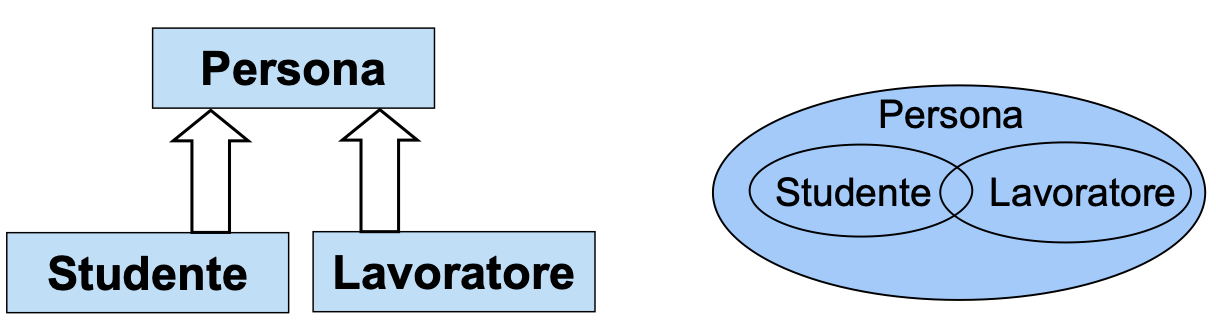
\includegraphics[width=0.9\linewidth]{../images/is1.png}
    %\caption{caption}
    %\label{label}
\end{figure}

\subsubsection*{Le entità figlie possono avere istanze in comune}
\textbf{Due entità figlie della stessa entità padre
possono avere istanze in comune.}
Ad esempio, una persona può essere contemporaneamente
Studente e Lavoratore.
Formalmente, se $I$ è un'istanza dello schema:
\[
\operatorname{istanze}(I,Studente)
\subseteq
\operatorname{istanze}(I,Persona)
\]
\[
\operatorname{istanze}(I,Lavoratore)
\subseteq
\operatorname{istanze}(I,Persona)
\]
ma è possibile che:
\[
\boxed{
\operatorname{istanze}(I,Studente)
\cap
\operatorname{istanze}(I,Lavoratore)
\neq \varnothing
}
\]
\textcolor{verdeScuro}{\textbf{Esempio.}}
Supponiamo:
\[
\operatorname{istanze}(I,Persona)=\{a,b,c,d\}
\]
\[
\operatorname{istanze}(I,Studente)=\{a,b\}
\]
\[
\operatorname{istanze}(I,Lavoratore)=\{b,c\}
\]
Allora:
\[
\operatorname{istanze}(I,Studente)
\cap
\operatorname{istanze}(I,Lavoratore)
=\{b\}
\]
Quindi $b$ è contemporaneamente Studente e Lavoratore.\\
\textbf{Attenzione:} questo non viola la regola secondo
cui ogni entità può avere al massimo un'entità padre.
Infatti, Studente e Lavoratore hanno entrambi Persona
come unico padre. È semplicemente la stessa istanza
che appartiene a due entità figlie differenti.
% ============================================================
% GENERALIZZAZIONE
% ============================================================
\subsection{Generalizzazione tra entità}
La \textbf{generalizzazione} è un costrutto del modello ER
che permette di rappresentare più sottoentità
(almeno due), appartenenti a una stessa entità padre,
distinte secondo un \textbf{unico criterio di classificazione}.\\
A differenza di semplici relazioni ISA,
nella generalizzazione considerata nel corso
le sottoentità sono \textbf{disgiunte a coppie}.
Questo significa che un'istanza dell'entità padre
può appartenere ad al massimo una delle sottoentità
della stessa generalizzazione.\\
\textcolor{verdeScuro}{\textbf{Esempio.}}
Supponiamo di classificare le Persone
in Uomo e Donna secondo il criterio adottato
dallo schema.\\
Le due sottoentità costituiscono una generalizzazione
di Persona.
Ogni Uomo è una Persona e ogni Donna è una Persona,
ma nessuna istanza può appartenere contemporaneamente
a entrambe le sottoentità di questa generalizzazione.
\subsubsection*{Differenza tra ISA e generalizzazione}
La distinzione fondamentale è:
\begin{itemize}
    \item \textbf{ISA:} due entità figlie della stessa
    entità padre possono avere istanze in comune.

    \item \textbf{Generalizzazione:} le sottoentità
    appartenenti alla stessa generalizzazione
    devono essere disgiunte a coppie.
\end{itemize}
\noindent
Inoltre, una generalizzazione può essere
\textbf{completa} oppure \textbf{non completa}.

\subsubsection*{Generalizzazione completa}
Una generalizzazione è \textbf{completa}
quando ogni istanza dell'entità padre appartiene
necessariamente a una delle sottoentità.
In altre parole, l'unione degli insiemi delle istanze
delle sottoentità coincide con l'insieme delle istanze
dell'entità padre.
\[
\boxed{
\bigcup_{i=1}^{n}
\operatorname{istanze}(I,E_i)
=
\operatorname{istanze}(I,F)
}
\]
dove $F$ è l'entità padre ed $E_1,\ldots,E_n$
sono le sottoentità.\\
\textcolor{verdeEsempio}{\textbf{Esempio.}}
Consideriamo una generalizzazione completa
di Persona nelle sottoentità Uomo e Donna.
Supponiamo:
\[
\operatorname{istanze}(I,Persona)=\{a,b,c,d\}
\]
\[
\operatorname{istanze}(I,Uomo)=\{a,c\}
\]
\[
\operatorname{istanze}(I,Donna)=\{b,d\}
\]
Abbiamo:
\[
\{a,c\}\cup\{b,d\}=\{a,b,c,d\}
\]
Quindi la generalizzazione è completa.
Inoltre:
\[
\{a,c\}\cap\{b,d\}=\varnothing
\]
Le sottoentità sono anche disgiunte.
\subsubsection*{Generalizzazione non completa}
Una generalizzazione è \textbf{non completa}
quando non è obbligatorio che ogni istanza
dell'entità padre appartenga a una sottoentità.
Formalmente, deve valere:
\[
\boxed{
\bigcup_{i=1}^{n}
\operatorname{istanze}(I,E_i)
\subseteq
\operatorname{istanze}(I,F)
}
\]
L'inclusione può essere stretta.\\
\textcolor{verdeEsempio}{\textbf{Esempio.}}
Consideriamo una generalizzazione non completa
di Persona nelle sottoentità Studente e Docente.
Supponiamo:
\[
\operatorname{istanze}(I,Persona)=\{a,b,c,d\}
\]
\[
\operatorname{istanze}(I,Studente)=\{a,b\}
\]
\[
\operatorname{istanze}(I,Docente)=\{c\}
\]
Allora:
\[
\{a,b\}\cup\{c\}=\{a,b,c\}
\]
e:
\[
\{a,b,c\}\subsetneq\{a,b,c,d\}
\]
L'istanza $d$ è una Persona,
ma non appartiene né a Studente né a Docente.
Questa situazione è consentita perché
la generalizzazione non è completa.\\
\textbf{Osservazione:} anche in una generalizzazione
non completa le sottoentità devono essere disgiunte.
La completezza riguarda la copertura dell'entità padre,
non la disgiunzione.
% ============================================================
% RAPPRESENTAZIONE GRAFICA
% ============================================================
\subsubsection*{Rappresentazione grafica della generalizzazione}
La generalizzazione viene rappresentata:
\begin{enumerate}
    \item Collegando le sottoentità mediante
    un unico arco di collegamento.

    \item Collegando tale arco all'entità padre
    attraverso una freccia.
\end{enumerate}
\noindent
La freccia cambia in base al tipo di generalizzazione:
\begin{itemize}
    \item \textbf{Completa:} freccia annerita.

    \item \textbf{Non completa:} freccia non annerita.
\end{itemize}
\noindent
\textcolor{verdeEsempio}{Esempio:} generalizzazione completa.
\begin{figure}[H]
    \centering  
    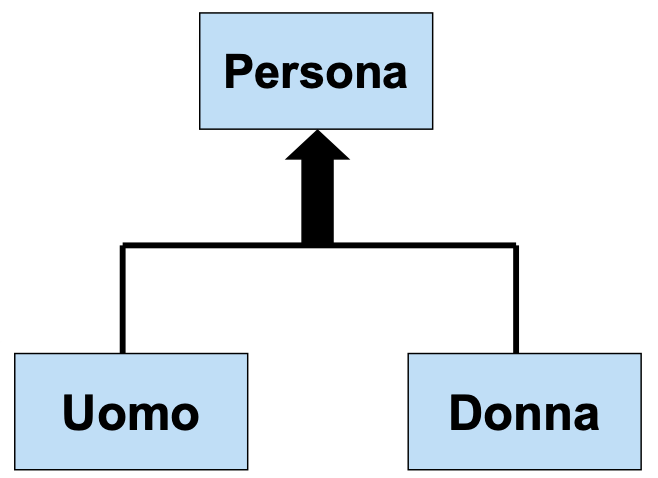
\includegraphics[width=0.4\linewidth]{../images/is2.png}
    %\caption{caption}
    %\label{label}
\end{figure}
\noindent
La freccia piena indica che tutte le Persone
appartengono a una delle sottoentità.\\
\textcolor{verdeEsempio}{Esempio:} generalizzazione non completa.
\begin{figure}[H]
    \centering  
    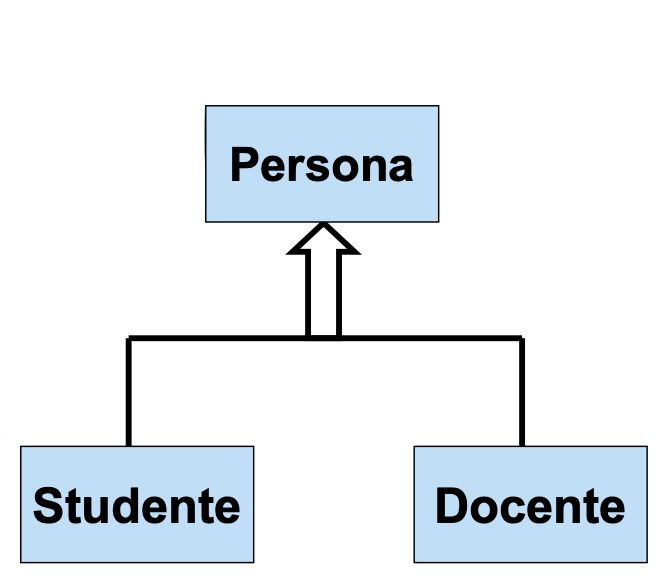
\includegraphics[width=0.4\linewidth]{../images/is3.png}
    %\caption{caption}
    %\label{label}
\end{figure}
\noindent
La freccia vuota indica che possono esistere
Persone che non sono né Studenti né Docenti.

% ============================================================
% SEMANTICA FORMALE
% ============================================================

\subsubsection*{Semantica della generalizzazione}

Consideriamo uno schema $S$ contenente
una generalizzazione tra:

\begin{itemize}
    \item un'entità padre $F$;
    \item le sottoentità $E_1,E_2,\ldots,E_n$,
    con $n>1$.
\end{itemize}
\noindent
Per ogni istanza $I$ dello schema $S$
devono essere rispettati i seguenti vincoli.\\
\textbf{1. Vincolo di inclusione}\\
Ogni sottoentità è in relazione ISA
con l'entità padre.
Quindi:
\[
\boxed{
\forall i\in\{1,\ldots,n\},
\quad
\operatorname{istanze}(I,E_i)
\subseteq
\operatorname{istanze}(I,F)
}
\]
\textbf{2. Vincolo di disgiunzione}\\
Due sottoentità distinte della stessa
generalizzazione non possono avere
istanze in comune.
\[
\boxed{
\forall i\neq k,
\quad
\operatorname{istanze}(I,E_i)
\cap
\operatorname{istanze}(I,E_k)
=
\varnothing
}
\]
\textbf{3. Vincolo di completezza}\\
Se la generalizzazione è completa,
deve valere anche:
\[
\boxed{
\bigcup_{i=1}^{n}
\operatorname{istanze}(I,E_i)
=
\operatorname{istanze}(I,F)
}
\]
Questo significa che ogni istanza
dell'entità padre deve appartenere
a una delle sottoentità.
\subsubsection*{Generalizzazione completa come partizione}
In matematica, una \textbf{partizione}
di un insieme è una famiglia di sottoinsiemi
non vuoti, disgiunti a coppie,
la cui unione coincide con l'insieme originale.\\
Uuna generalizzazione completa determina una partizione dell'entità padre
nel senso che le sottoentità sono disgiunte
e coprono completamente l'entità padre.
In particolare:
\[
\operatorname{istanze}(I,F)
=
\operatorname{istanze}(I,E_1)
\cup \cdots \cup
\operatorname{istanze}(I,E_n)
\]
con intersezioni a coppie vuote.
% ============================================================
% GENERALIZZAZIONE ED EREDITARIETÀ
% ============================================================
\subsubsection*{Generalizzazione ed ereditarietà}
Il principio di ereditarietà, già introdotto
per la relazione ISA, vale anche
per le generalizzazioni.\\
Ogni sottoentità eredita:
\begin{itemize}
    \item tutti gli attributi dell'entità padre;
    \item la possibilità di partecipare
    alle relazioni dell'entità padre;
    \item i vincoli associati alle proprietà ereditate.
\end{itemize}
\noindent
Le proprietà ereditate non vengono ripetute
esplicitamente nel diagramma.\\
\textcolor{verdeEsempio}{\textbf{Esempio.}}
Consideriamo una generalizzazione di Persona
nelle sottoentità Studente e Docente.
Persona possiede:
\begin{itemize}
    \item Cognome;
    \item Età;
    \item la relazione Sede con Città.
\end{itemize}
\noindent
Studente possiede inoltre Matricola,
mentre Docente partecipa alla relazione
Insegna con Corso.
\begin{center}
\begin{tikzpicture}[
    entita/.style={
        draw, rectangle, fill=lightblue,
        minimum width=2.3cm, minimum height=0.9cm
    },
    scala/.style={scale=0.85, transform shape}
]
\begin{scope}[scala]

% Entità
\node[entita] (p) at (0,3.5) {Persona};
\node[entita] (s) at (-3,0) {Studente};
\node[entita] (d) at (3,0) {Docente};
\node[entita] (c) at (7,3.5) {Città};
\node[entita] (co) at (9,0) {Corso};

% Generalizzazione
\draw[thick] (s.north) -- (-3,1.4)
    -- (3,1.4) -- (d.north);

\draw[thick] (0,1.4) -- (0,2.65);
\draw[thick, fill=white]
    (-0.25,2.65) -- (0,3.05) --
    (0.25,2.65) -- cycle;

% Relazione Sede: rombo manuale
\draw[thick, fill=lightblue]
    (3.5,4.1) -- (4.6,3.5) --
    (3.5,2.9) -- (2.4,3.5) -- cycle;
\node at (3.5,3.5) {Sede};

\draw[thick] (p.east) -- (2.4,3.5);
\draw[thick] (4.6,3.5) -- (c.west);

% Relazione Insegna: rombo manuale
\draw[thick, fill=lightblue]
    (6,0.6) -- (7.2,0) --
    (6,-0.6) -- (4.8,0) -- cycle;
\node at (6,0) {Insegna};

\draw[thick] (d.east) -- (4.8,0);
\draw[thick] (7.2,0) -- (co.west);

% Attributi Persona
\draw (p.north west) -- (-1.1,4.7);
\draw (p.north east) -- (1.1,4.7);
\draw[fill=white] (-1.1,4.7) circle (0.09);
\draw[fill=white] (1.1,4.7) circle (0.09);
\node[above] at (-1.1,4.7) {Cognome};
\node[above] at (1.1,4.7) {Età};

% Attributo Studente
\draw (s.south) -- (-3,-1);
\draw[fill=white] (-3,-1) circle (0.09);
\node[below] at (-3,-1) {Matricola};

% Attributo Città
\draw (c.north) -- (7,4.7);
\draw[fill=white] (7,4.7) circle (0.09);
\node[above] at (7,4.7) {Nome};

% Attributo Corso
\draw (co.south) -- (9,-1);
\draw[fill=white] (9,-1) circle (0.09);
\node[below] at (9,-1) {Codice};

\end{scope}
\end{tikzpicture}
\end{center}
Da questo schema segue che:
\begin{itemize}
    \item ogni Studente possiede Cognome, Età
    e Matricola;

    \item ogni Docente possiede Cognome ed Età;

    \item Studente e Docente possono partecipare
    alla relazione Sede, perché ereditata da Persona;

    \item Docente partecipa anche alla relazione
    Insegna, definita specificamente
    per questa sottoentità.
\end{itemize}

% ============================================================
% REGOLE
% ============================================================

\subsubsection*{Regole sulle generalizzazioni}

Nel modello ER utilizzato nel corso
continua a valere la seguente regola:
\[
\boxed{
\text{Ogni entità può avere al massimo
un'entità padre diretta}
}
\]
Questa regola vale considerando insieme
sia le relazioni ISA sia le generalizzazioni.
Pertanto, un'entità non può:
\begin{itemize}
    \item essere figlia di due entità diverse
    mediante due relazioni ISA;

    \item appartenere a una generalizzazione
    e avere contemporaneamente un altro padre
    mediante ISA;

    \item appartenere a due generalizzazioni
    con entità padre differenti.
\end{itemize}
\noindent
\textcolor{verdeEsempio}{Esempio} di schema scorretto.\\
\begin{figure}[H]
    \centering  
    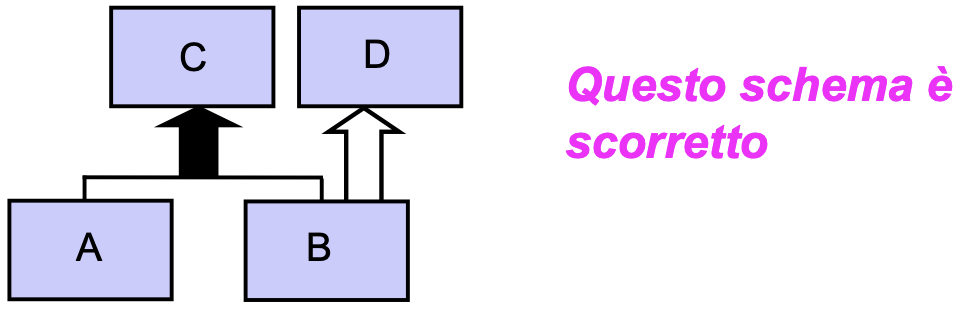
\includegraphics[width=0.4\linewidth]{../images/is5.png}
    %\caption{caption}
    %\label{label}
\end{figure}

% ============================================================
% ESERCIZIO 13
% ============================================================
\subsubsection*{Esercizio 13: relazione ISA e generalizzazioni}
Consideriamo le entità:
\begin{itemize}
    \item Studente, con attributi CodFisc e Matricola;
    \item Lavoratore, con attributi CodFisc e Salario;
    \item StudenteLavoratore, con attributo Esenzione.
\end{itemize}
\noindent
Si vuole rappresentare il fatto che
uno StudenteLavoratore sia contemporaneamente
uno Studente e un Lavoratore.
Una prima idea potrebbe essere:
\[
\text{StudenteLavoratore ISA Studente}
\]
\[
\text{StudenteLavoratore ISA Lavoratore}
\]
\subsubsection*{Soluzione 1: suddivisione in tre sottoentità}
La prima soluzione consiste nell'introdurre
un'entità padre:
\[
\text{StudenteOLavoratore}
\]
che rappresenta tutte le persone che sono
studenti, lavoratori oppure entrambe le cose.
Si definisce una generalizzazione completa
nelle tre sottoentità:
\begin{itemize}
    \item StudenteNonLav;
    \item StudenteLavoratore;
    \item LavoratoreNonSt.
\end{itemize}


\begin{figure}[H]
    \centering  
    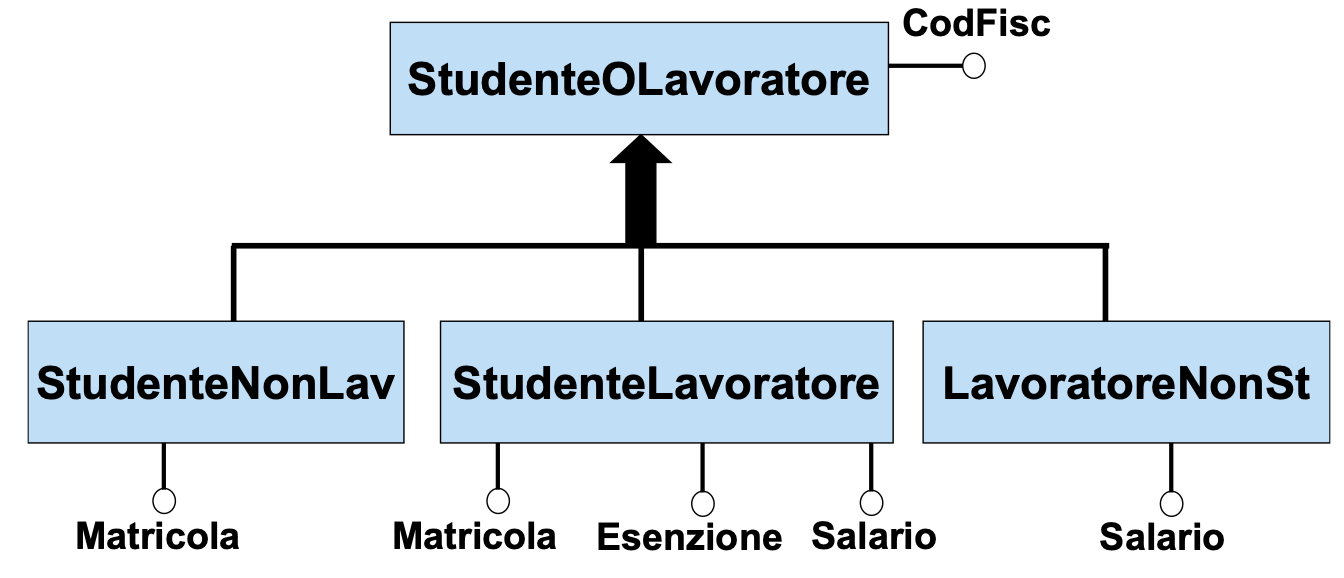
\includegraphics[width=0.5\linewidth]{../images/is6.png}
    %\caption{caption}
    %\label{label}
\end{figure}
\noindent L'attributo CodFisc viene associato
all'entità padre StudenteOLavoratore,
perché appartiene a tutte e tre le categorie.
\noindent
\textbf{Perché questa soluzione funziona?}\\
Le tre sottoentità sono disgiunte.
Inoltre, la generalizzazione è completa:
\[
\begin{aligned}
&\operatorname{istanze}(I,StudenteNonLav)
\\
&\quad\cup
\operatorname{istanze}(I,StudenteLavoratore)
\\
&\quad\cup
\operatorname{istanze}(I,LavoratoreNonSt)
\\
&=
\operatorname{istanze}(I,StudenteOLavoratore)
\end{aligned}
\]
\textbf{Svantaggio:} se nello schema originale
esistevano sottoentità di Studente o Lavoratore,
potrebbe essere necessario suddividerle
tra le nuove categorie.
Questo può rendere lo schema più complesso.
\subsubsection*{Soluzione 2: mantenere Studente come entità}
La seconda soluzione mantiene Studente
come entità specifica e introduce
LavoratoreNonSt come altra sottoentità
di StudenteOLavoratore.
Si ottiene una generalizzazione completa:
\[
\text{StudenteOLavoratore}
\]
con sottoentità:
\[
\text{Studente},\quad
\text{LavoratoreNonSt}
\]
e
\[
\text{StudenteLavoratore ISA Studente}
\]
\begin{figure}[H]
    \centering  
    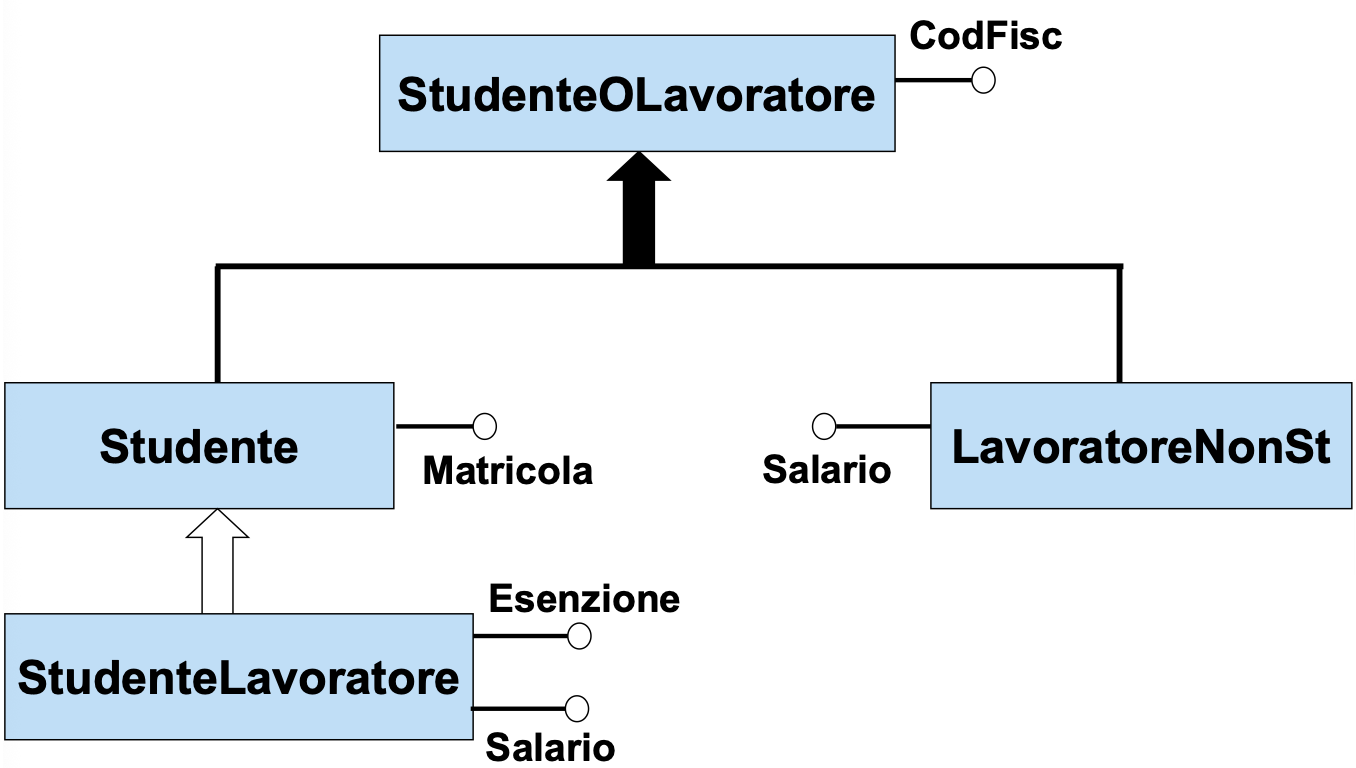
\includegraphics[width=0.5\linewidth]{../images/is4.png}
    %\caption{caption}
    %\label{label}
\end{figure}
\noindent
StudenteLavoratore eredita automaticamente
Matricola da Studente e CodFisc
da StudenteOLavoratore.\\
\textbf{Vantaggio:} si mantiene l'entità Studente
e quindi non è necessario suddividere
le sue eventuali sottoentità.\\
\textbf{Svantaggio:} eventuali sottoentità
di Lavoratore potrebbero richiedere
una ristrutturazione.

\subsubsection*{Soluzione 3: mantenere Lavoratore come entità}
Si introduce una generalizzazione completa
di StudenteOLavoratore nelle sottoentità:
\[
\text{Lavoratore},\quad
\text{StudenteNonLav}
\]
Inoltre, si definisce:
\[
\text{LavoratoreStudente ISA Lavoratore}
\]
\begin{figure}[H]
    \centering  
    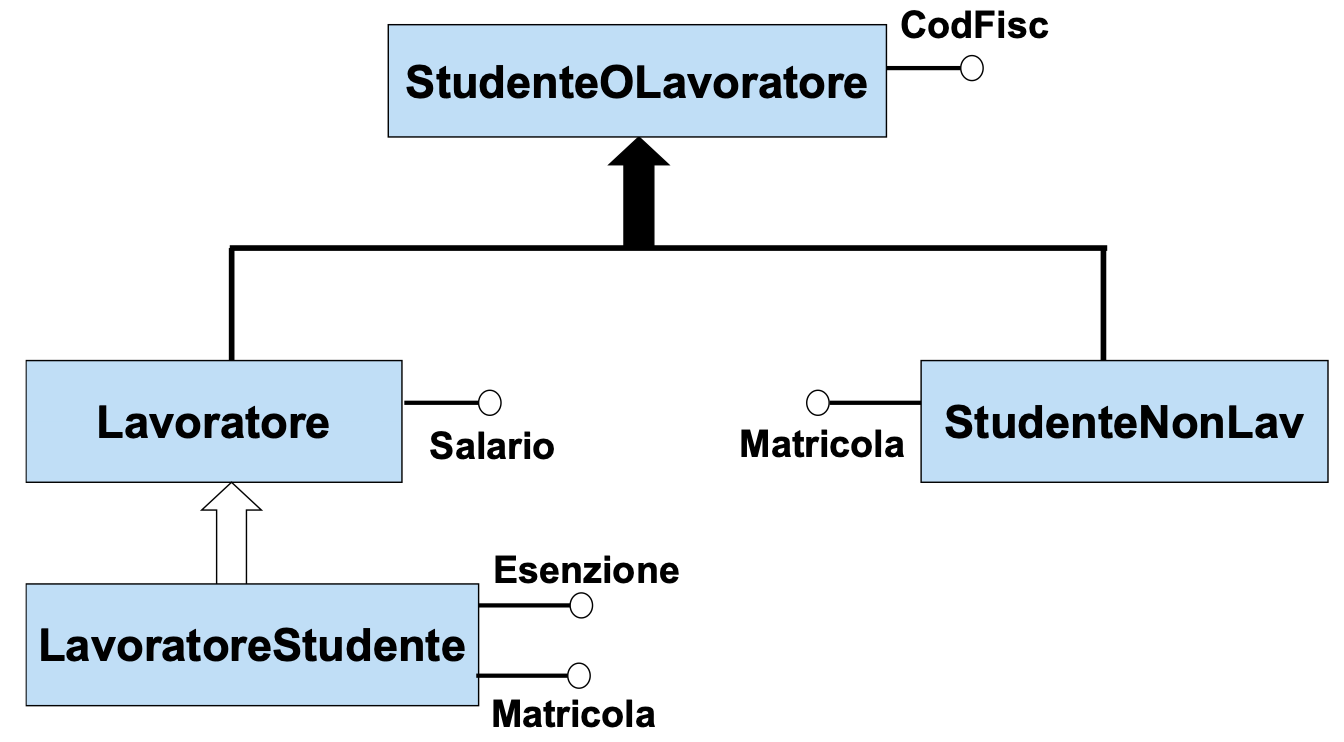
\includegraphics[width=0.5\linewidth]{../images/is7.png}
    %\caption{caption}
    %\label{label}
\end{figure}
\noindent
LavoratoreStudente eredita automaticamente
Salario da Lavoratore e CodFisc
da StudenteOLavoratore.\\
\textbf{Vantaggio:} viene mantenuta
l'entità Lavoratore e non è necessario
suddividere le sue eventuali sottoentità.\\
\textbf{Svantaggio:} eventuali sottoentità
di Studente potrebbero richiedere
una ristrutturazione.\medskip\\
\textbf{Conclusione.}
Le tre soluzioni permettono di evitare
l'ereditarietà multipla e di rappresentare
sostanzialmente la stessa realtà.
La scelta dipende dalla struttura
del resto dello schema e da quali entità
si desidera mantenere senza suddividerle.


% ==========================================================
% DIVERSE GENERALIZZAZIONI DELLA STESSA ENTITÀ
% ==========================================================

\subsection*{Diverse generalizzazioni della stessa entità}

Una stessa entità può essere \textbf{padre di più generalizzazioni}, purché queste rappresentino criteri differenti di classificazione delle sue istanze.\\
Ogni generalizzazione considera quindi una caratteristica diversa degli oggetti appartenenti all'entità padre.\medskip\\
\textcolor{verdeEsempio}{\textbf{Esempio. }}Consideriamo l'entità Persona.\\
Possiamo classificare le persone secondo due criteri:
\begin{itemize}
    \item \textbf{Sesso}: Uomo e Donna.
    \item \textbf{Condizione occupazionale}: Impiegato e Studente.
\end{itemize}
\noindent
La prima generalizzazione è \textbf{completa}, mentre la seconda è \textbf{non completa}.\\
Inoltre, le due generalizzazioni sono indipendenti: una persona può essere contemporaneamente Uomo e Studente oppure Donna e Impiegato.
\begin{figure}[H]
    \centering  
    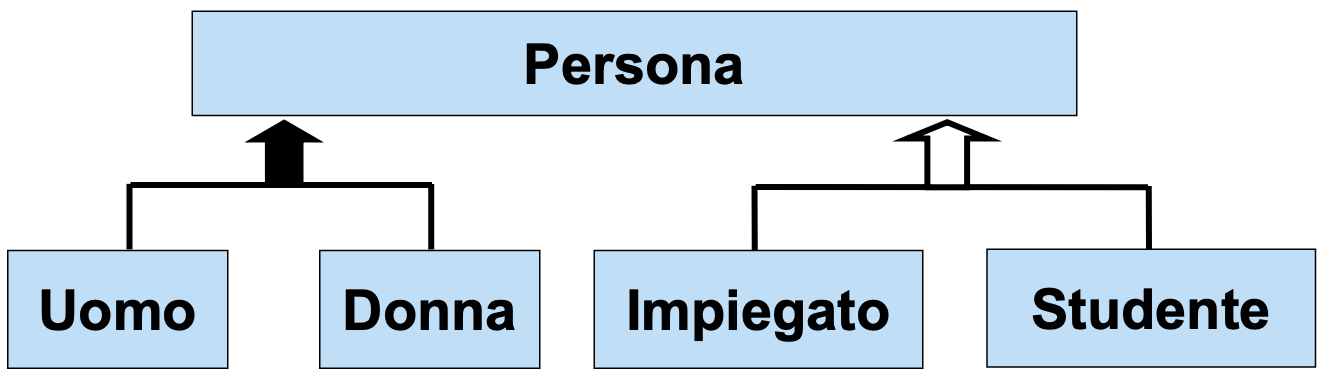
\includegraphics[width=0.5\linewidth]{../images/gen1.png}
    %\caption{caption}
    %\label{label}
\end{figure}

% ==========================================================
% DIFFERENZA TRA ISA E GENERALIZZAZIONE
% ==========================================================

\subsection{Differenza tra relazioni ISA e generalizzazioni}

La relazione ISA e la generalizzazione esprimono entrambe una relazione di specializzazione, ma hanno un significato differente.

\subsubsection*{Relazione ISA}

Una relazione ISA collega \textbf{una singola entità figlia} alla sua entità padre.\\
Esprime semplicemente il fatto che ogni istanza dell'entità figlia è anche un'istanza dell'entità padre.

\[
\operatorname{istanze}(I,E)
\subseteq
\operatorname{istanze}(I,F)
\]
dove $E$ è la figlia e $F$ è il padre. Non impone, da sola, alcun vincolo di disgiunzione rispetto ad altre sottoentità.

\subsubsection*{Generalizzazione}

Una generalizzazione raggruppa \textbf{almeno due sottoentità} che derivano da uno stesso criterio di classificazione dell'entità padre.\\
Le sottoentità della stessa generalizzazione sono disgiunte a coppie.\medskip\\
\textcolor{verdeEsempio}{\textbf{Esempio. }}
Supponiamo che Persona abbia le sottoentità Uomo, Donna, Impiegato e Sportivo.
\begin{figure}[H]
    \centering  
    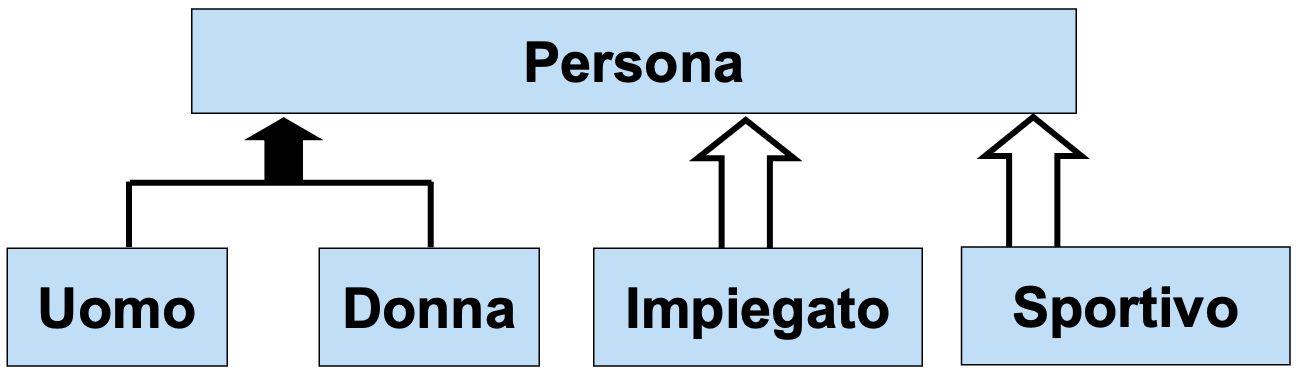
\includegraphics[width=0.5\linewidth]{../images/gen2.png}
    %\caption{caption}
    %\label{label}
\end{figure}
\noindent
Un impiegato può anche essere sportivo, mentre una stessa persona non può appartenere contemporaneamente a Uomo e Donna nel modello rappresentato.

\[
\begin{aligned}
Uomo &\cap Donna = \varnothing\\
Impiegato &\cap Sportivo
\text{ può essere non vuoto}
\end{aligned}
\]

% ==========================================================
% ESERCIZIO 14
% ==========================================================

\subsection*{Esercizio: progettazione delle generalizzazioni}
\subsubsection*{Specifiche}

Si vuole rappresentare uno schema concettuale in cui:

\begin{itemize}
    \item Ogni persona possiede un codice fiscale e un'età.
    \item Gli uomini possiedono anche una posizione militare.
    \item Le donne possiedono anche un numero di maternità.
    \item Gli impiegati possiedono uno stipendio e possono essere segretari, direttori oppure progettisti.
    \item Alcuni progettisti sono responsabili di progetto.
    \item Gli studenti possiedono una matricola e non possono essere impiegati.
    \item Esistono persone che non sono né studenti né impiegati.
\end{itemize}
\noindent
L'obiettivo è individuare le entità, gli attributi, le generalizzazioni e le relazioni ISA.

\subsubsection*{Soluzione}
\begin{figure}[H]
    \centering  
    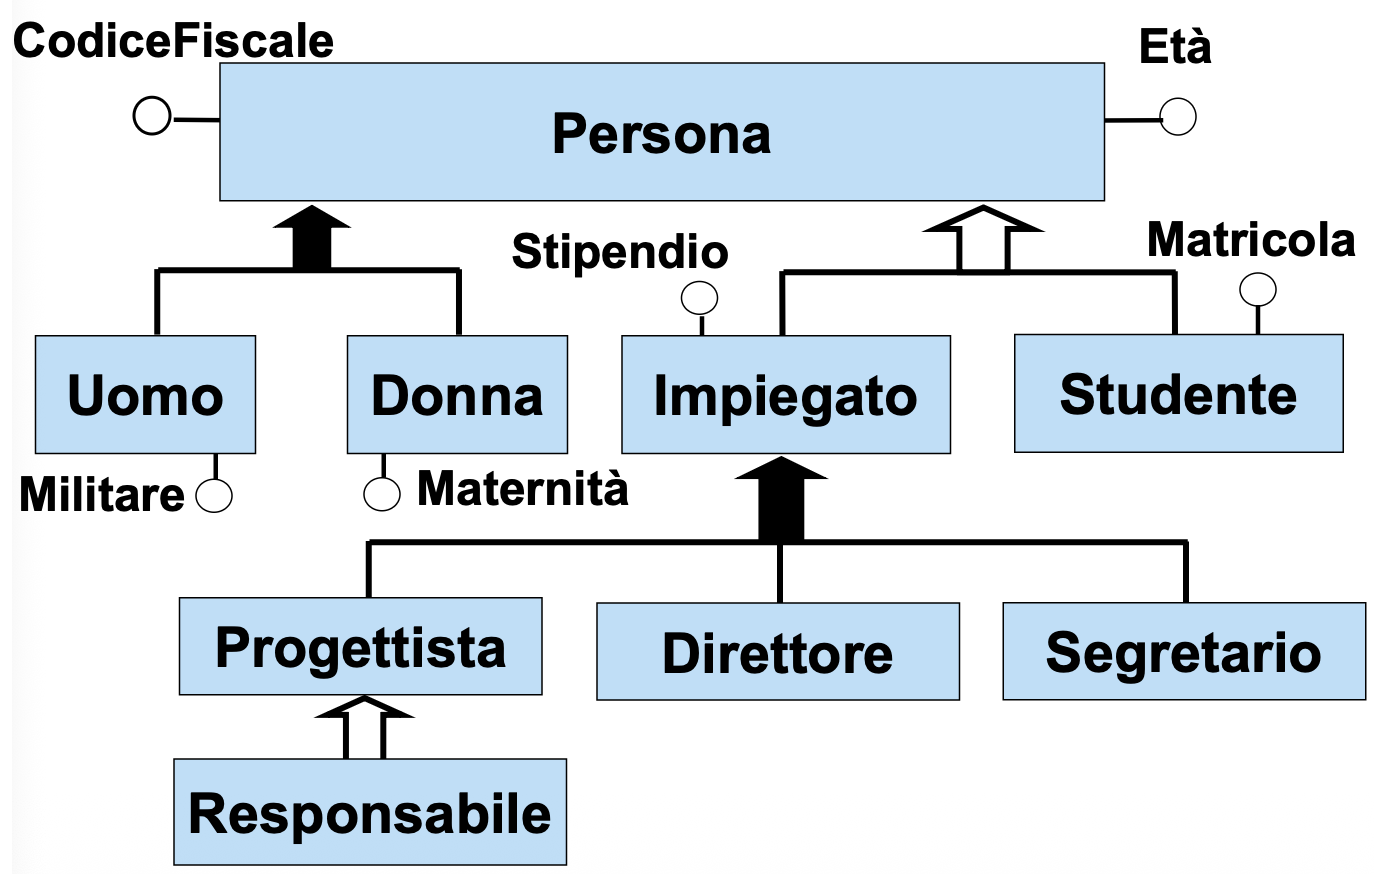
\includegraphics[width=0.5\linewidth]{../images/gen3.png}
    %\caption{caption}
    %\label{label}
\end{figure}
% ==========================================================
% GRAFO DELLE GERARCHIE
% ==========================================================

\subsection{Grafo delle gerarchie}

A ogni schema concettuale $S$ è possibile associare un \textbf{grafo delle gerarchie}, che rappresenta le relazioni di specializzazione tra entità e tra relazioni.

\subsubsection*{Costruzione del grafo}

\begin{enumerate}
    \item Si crea un nodo per ogni entità e per ogni relazione dello schema.
    \item Si traccia un arco diretto dall'entità figlia verso l'entità padre per ogni ISA o generalizzazione.
    \item Si applica lo stesso procedimento alle relazioni, quando sono presenti ISA o generalizzazioni tra relazioni.
    \item Se si formano cicli, tutti i nodi appartenenti a ciascun ciclo vengono collassati in un unico nodo.
\end{enumerate}
\noindent
Gli archi sono quindi orientati \textbf{dalla specializzazione verso la generalizzazione}.

\subsubsection*{Concetto di antenato}

Un'entità $G$ è detta \textbf{antenata} di un'entità $E$ se nel grafo delle gerarchie esiste un cammino diretto da $E$ a $G$.\\
Il cammino può avere anche lunghezza zero: di conseguenza, ogni entità è antenata di se stessa.\medskip\\
\textcolor{verdeEsempio}{\textbf{Esempio. }} Consideriamo la gerarchia:
\[
Responsabile
\longrightarrow
Progettista
\longrightarrow
Impiegato
\longrightarrow
Persona
\]
\noindent
In questo caso:
\begin{itemize}
    \item Progettista è antenata di Responsabile.
    \item Impiegato è antenata di Responsabile.
    \item Persona è antenata di Responsabile.
    \item Responsabile è antenata di se stessa.
\end{itemize}

% ==========================================================
% ENTITÀ DISGIUNTE
% ==========================================================

\subsection{Entità disgiunte}
Due entità $E$ e $F$ sono \textbf{disgiunte} se non condividono alcuna istanza, in ogni possibile istanza dello schema.

\[
\operatorname{istanze}(I,E)
\cap
\operatorname{istanze}(I,F)
=
\varnothing
\]

\noindent
La disgiunzione può essere stabilita direttamente, oppure derivata dalla struttura delle generalizzazioni.

\subsubsection*{L'entità speciale TOP}

Per formulare una regola generale, si introduce un'entità fittizia chiamata \textbf{TOP}.\\
Le entità che non hanno un padre nel grafo delle gerarchie vengono considerate sottoentità di una generalizzazione completa con padre TOP.
Rappresenta quindi l'insieme di tutti gli oggetti presenti nelle entità dello schema.

\subsubsection*{Regola generale di disgiunzione}

Due entità distinte $E$ e $F$ sono disgiunte, secondo i vincoli della gerarchia, se esistono due entità $G$ e $H$ tali che:

\begin{enumerate}
    \item $G$ e $H$ sono sottoentità diverse della stessa generalizzazione, quindi sono disgiunte.
    \item $G$ è antenata di $E$.
    \item $H$ è antenata di $F$.
\end{enumerate}
\noindent
In altre parole, \textbf{due entità sono disgiunte quando discendono da due rami incompatibili di una stessa generalizzazione}.

% ==========================================================
% ISA TRA RELAZIONI
% ==========================================================

\subsection{Relazioni ISA tra relazioni}

La relazione ISA può essere definita non soltanto tra entità, ma anche tra \textbf{relazioni}.\\
In questo caso una relazione più specifica è figlia di una relazione più generale.
\subsubsection*{Condizioni necessarie}
Siano $R$ la relazione figlia e $Q$ la relazione padre.\\
Per poter definire:

\[
R\ ISA\ Q
\]
devono essere rispettate due condizioni:
\begin{enumerate}
    \item $R$ e $Q$ devono avere \textbf{lo stesso insieme di ruoli}, e quindi lo stesso grado.
    \item Per ogni ruolo, l'entità corrispondente in $R$ deve essere in relazione ISA, eventualmente transitiva o riflessiva, con l'entità corrispondente in $Q$.
\end{enumerate}
\subsubsection*{Semantica}

La semantica è analoga a quella dell'ISA tra entità:

\[
\operatorname{istanze}(I,R)
\subseteq
\operatorname{istanze}(I,Q)
\]

\noindent
Ogni tupla appartenente alla relazione figlia deve quindi appartenere anche alla relazione padre, considerando gli stessi ruoli.\medskip\\
\textcolor{verdeEsempio}{\textbf{Esempio. }} Lavora e Dirige
\begin{figure}[H]
    \centering  
    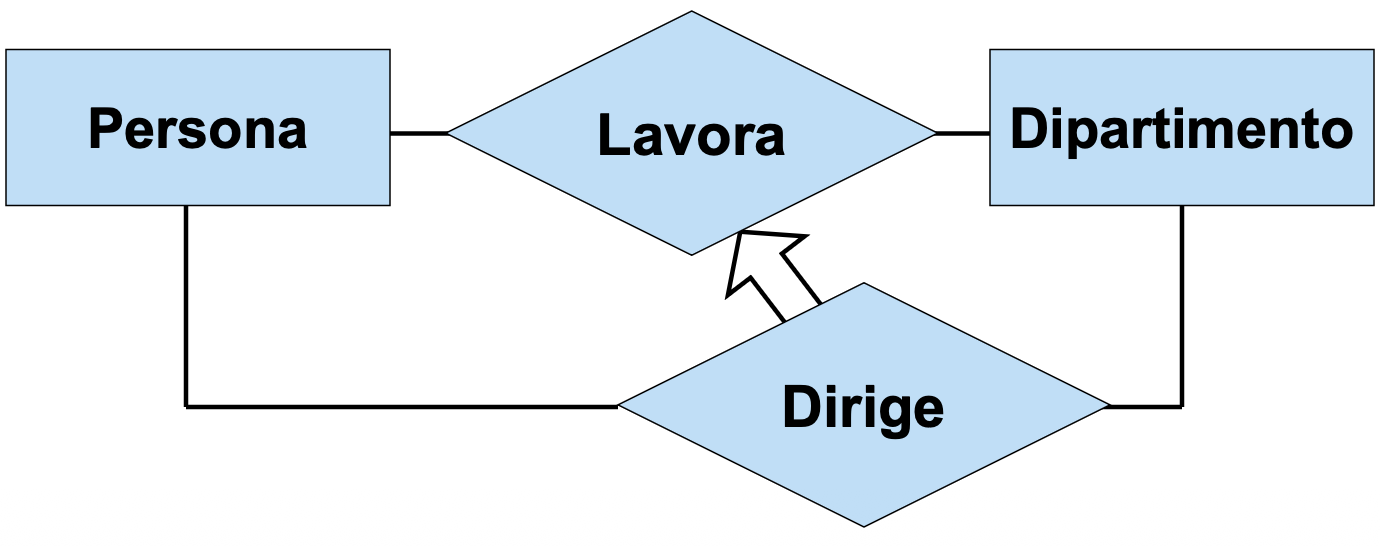
\includegraphics[width=0.4\linewidth]{../images/relgen1.png}
    %\caption{caption}
    %\label{label}
\end{figure}
\noindent
La regola aziendale stabilisce che chi dirige un dipartimento deve anche lavorare nello stesso dipartimento.

\[
Dirige\ ISA\ Lavora
\]
\noindent
Se Mario dirige il dipartimento Informatica, allora Mario deve anche lavorare nel dipartimento Informatica.\\
Non vale necessariamente il contrario: chi lavora in un dipartimento non deve per forza dirigerlo.

% ==========================================================
% ISA TRA RELAZIONI CON ENTITÀ SPECIALIZZATE
% ==========================================================

\subsubsection*{ISA tra relazioni con entità specializzate}

Le relazioni ISA possono coinvolgere anche entità diverse, purché siano compatibili con la gerarchia ISA.\medskip\\
\textcolor{verdeEsempio}{\textbf{Esempio. }} Nel caso in cui dei direttori si voglia avere attributi specifici, per esempio Età, che non appartengono necessariamente all'entità Persona nel particolare schema considerato. 
\begin{figure}[H]
    \centering  
    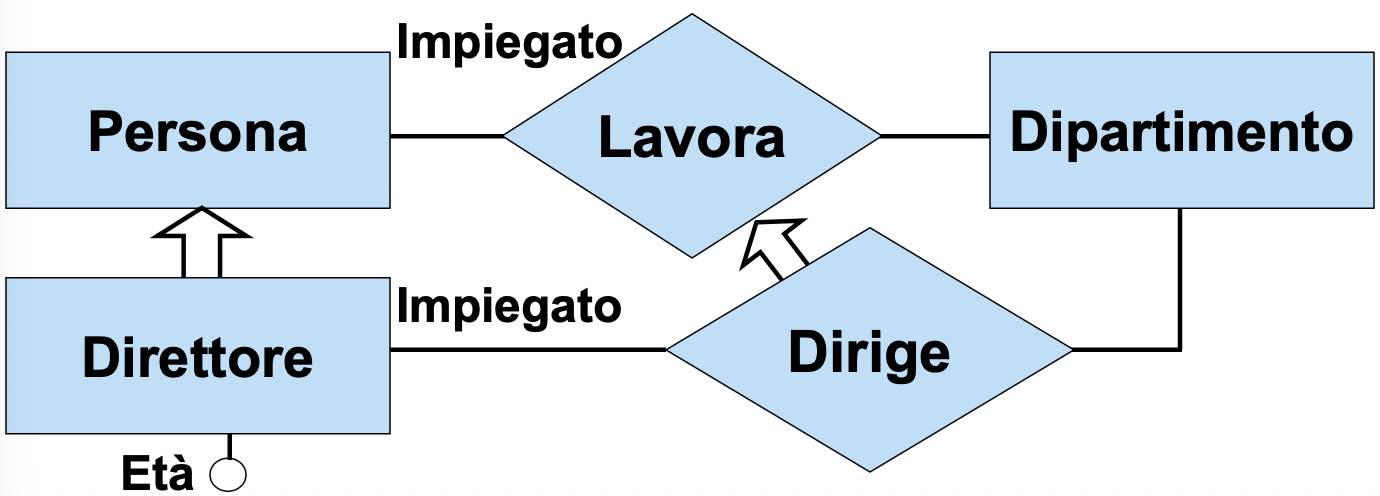
\includegraphics[width=0.5\linewidth]{../images/relgen2.png}
    %\caption{caption}
    %\label{label}
\end{figure}
\noindent
\textbf{Importante:} il nome del ruolo deve essere lo stesso in entrambe le relazioni.\\
Il fatto che due relazioni colleghino entità compatibili non è sufficiente se i ruoli sono differenti.

% ==========================================================
% GENERALIZZAZIONI TRA RELAZIONI
% ==========================================================

\subsubsection{Generalizzazioni tra relazioni}
Come per le entità, anche le relazioni possono essere organizzate in generalizzazioni.
Una relazione padre viene specializzata in più relazioni figlie, che rappresentano modalità alternative dello stesso collegamento.\medskip\\
\textcolor{verdeEsempio}{\textbf{Esempio. }}Un impiegato può lavorare a un progetto in modalità tradizionale oppure a distanza.
Definiamo:
\begin{figure}[H]
    \centering  
    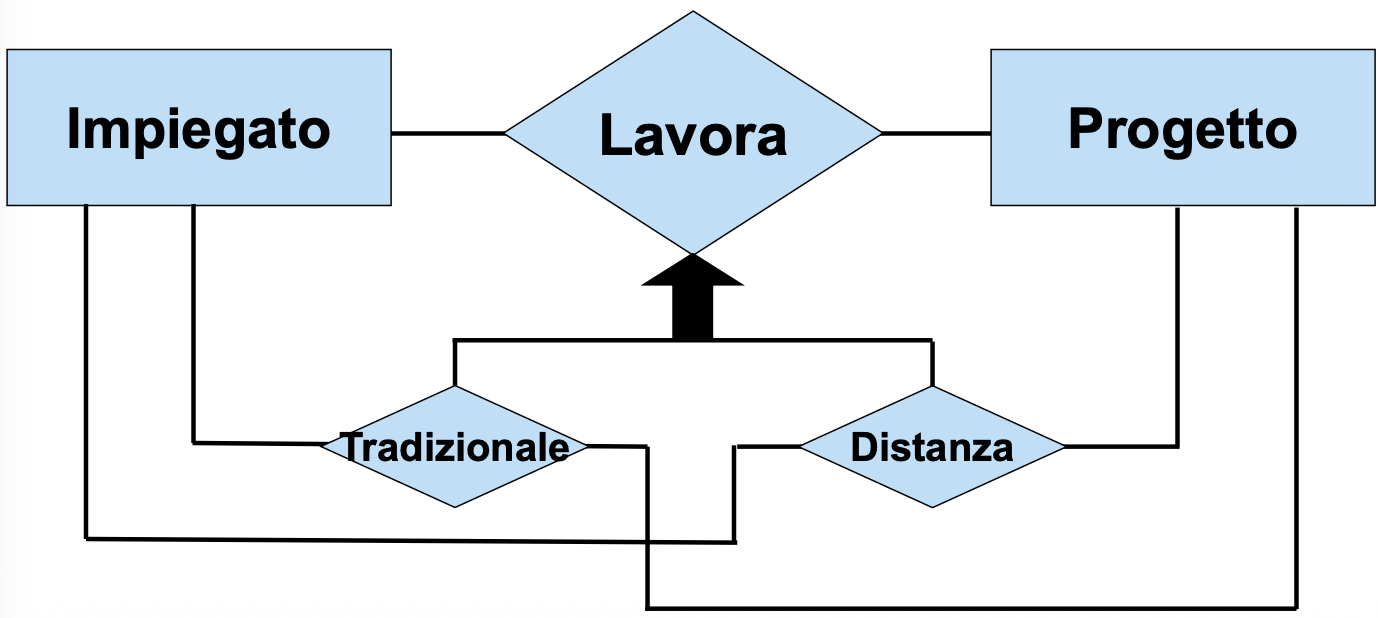
\includegraphics[width=0.5\linewidth]{../images/relgen3.png}
    %\caption{caption}
    %\label{label}
\end{figure}
\noindent
Le due relazioni figlie appartengono alla stessa generalizzazione di Lavora.

% ==========================================================
% ERRORI FREQUENTI
% ==========================================================

\subsection*{Errori frequenti nelle ISA tra relazioni}

Non ogni collegamento tra due relazioni può essere rappresentato mediante ISA.\\
È necessario verificare sia la compatibilità delle entità sia l'identità dei ruoli.

\subsubsection*{Errore 1: ruoli differenti}
\begin{figure}[H]
      
    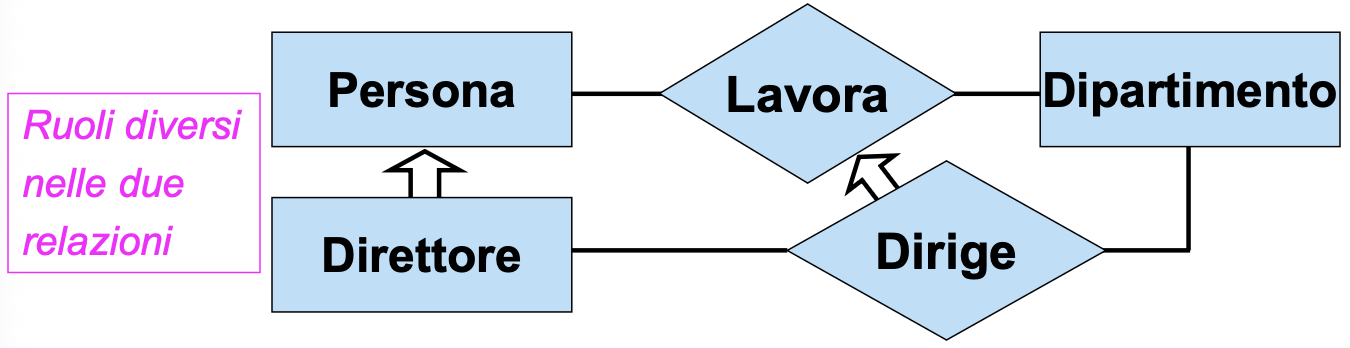
\includegraphics[width=0.5\linewidth]{../images/relgen4.png}
    %\caption{caption}
    %\label{label}
\end{figure}
\noindent
Anche se Direttore è una sottoentità di Persona, l'ISA tra relazioni non è ammessa, perché \textbf{i ruoli non coincidono}.

\subsubsection*{Errore 2: entità non collegate da ISA}
\begin{figure}[H]
      
    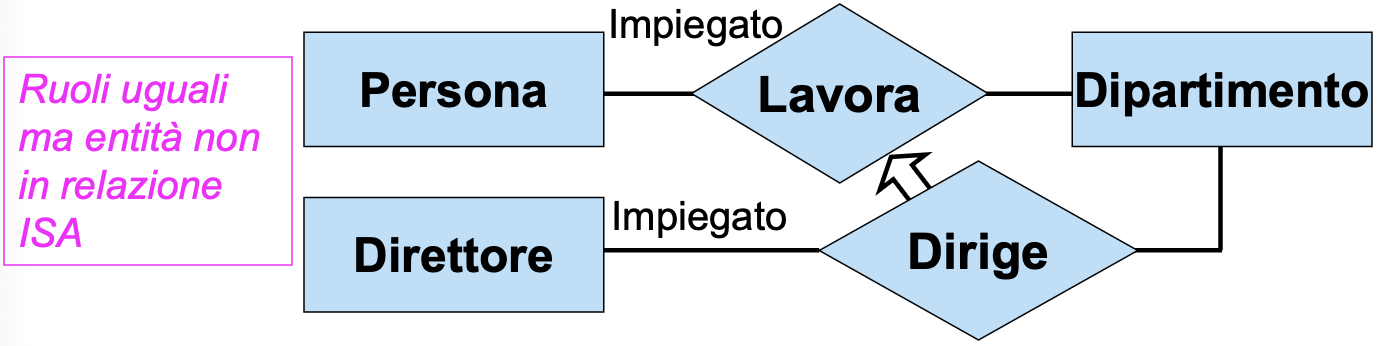
\includegraphics[width=0.5\linewidth]{../images/relgen5.png}
    %\caption{caption}
    %\label{label}
\end{figure}
\noindent
L'ISA tra relazioni non è ammessa, perchè non sappiamo se ogni direttore sia anche una persona secondo i vincoli dello schema.\medskip\\
\textbf{Attenzione. }Al contrario delle entità, due relazioni che non hanno padre nello schema \textbf{non sono disgiunte}.

\subsection{Vincoli di integrità nel modello ER}

Un \textbf{vincolo di integrità} è una regola che si esprime sullo
\textbf{schema} (livello intensionale), e che specifica una
condizione che deve valere \textbf{per ogni istanza} dello schema (livello estensionale).\\
In altre parole, un vincolo stabilisce quali dati e quali associazioni
sono ammessi nel database.\\
Nel modello ER distinguiamo quattro categorie principali:
\begin{itemize}
    \item \textbf{Vincoli di cardinalità sulle relazioni}: stabiliscono
    quante volte un'entità può partecipare a una relazione.
    \item \textbf{Vincoli di cardinalità sugli attributi}: stabiliscono
    quanti valori può assumere un attributo.
    \item \textbf{Vincoli di identificazione}: permettono di identificare
    univocamente le istanze di entità e relazioni.
    \item \textbf{Altri vincoli (esterni)}: esprimono condizioni aggiuntive
    non rappresentate direttamente dai vincoli precedenti.
\end{itemize}
\noindent
\textcolor{verdeEsempio}{\textbf{Esempio}}\\
Se nello schema è stabilito che ogni impiegato deve avere almeno
un incarico, non può esistere un'istanza valida del database
contenente un impiegato senza incarichi.

\subsection{Vincoli di cardinalità sulle relazioni}

Un \textbf{vincolo di cardinalità} è associato a un ruolo $U$
di un'entità $E$ in una relazione $R$.\\
Esso specifica il \textbf{numero minimo e massimo di istanze
della relazione} a cui può partecipare ogni istanza dell'entità
nel ruolo considerato.\\
Questi vincoli servono quindi a precisare il significato
delle relazioni e a limitare le associazioni ammesse.

\subsubsection*{Sintassi dei vincoli di cardinalità}

Un vincolo di cardinalità si rappresenta mediante una coppia:

\[
\boxed{(x,y)}
\]
dove:
\begin{itemize}
    \item $x$ è la \textbf{cardinalità minima}, cioè un intero
    maggiore o uguale a zero;
    \item $y$ è la \textbf{cardinalità massima}, cioè un intero
    positivo maggiore o uguale a $x$, oppure il simbolo $n$.
\end{itemize}
\noindent
\begin{figure}[H]
    \centering  
    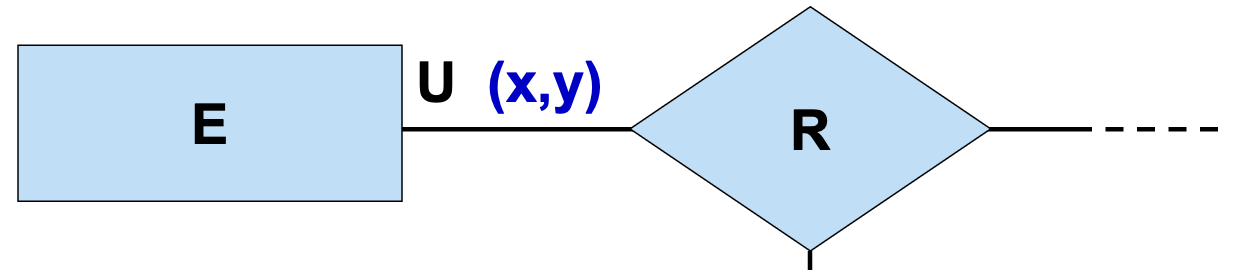
\includegraphics[width=0.5\linewidth]{../images/car1.png}
    %\caption{caption}
    %\label{label}
\end{figure}
\noindent
Il simbolo $n$ indica che \textbf{non viene imposto un limite
massimo prefissato} al numero di partecipazioni.

\subsubsection*{Semantica dei vincoli di cardinalità}

Consideriamo un'entità $E$ che partecipa a una relazione $R$
attraverso il ruolo $U$, con cardinalità $(x,y)$.\\
In ogni istanza valida $I$ dello schema, \textbf{ogni elemento
$e$ di $E$ deve partecipare alla relazione $R$ almeno $x$
volte e al massimo $y$ volte}, se $y$ è finito.\\
Indicando con $N_U(e)$ il numero di istanze di $R$
in cui compare $e$ nel ruolo $U$, si ha:

\[
\boxed{x \leq N_U(e) \leq y}
\]
Se invece $y=n$, è richiesto soltanto che:

\[
\boxed{N_U(e)\geq x}
\]
\textbf{Attenzione:} il vincolo è scritto su un ruolo della relazione,
ma deve essere verificato per \textbf{tutte le istanze dell'entità}
associata a quel ruolo, comprese quelle che non partecipano
ad alcuna istanza della relazione.

\subsubsection*{Esempio di vincoli di cardinalità}
Consideriamo la relazione \textbf{Assegnazione} tra
\textbf{Impiegato} e \textbf{Incarico}.\\
Le specifiche sono:
\begin{itemize}
    \item Ogni impiegato deve avere \textbf{da 1 a 5 incarichi}.
    \item Ogni incarico può essere assegnato ad
    \textbf{al massimo 50 impiegati}.
\end{itemize}
\noindent
Lo schema ER è:
\begin{figure}[H]
    \centering  
    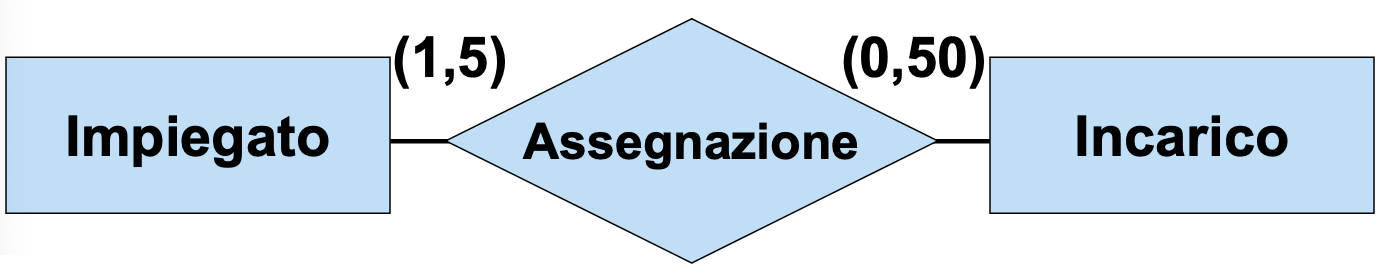
\includegraphics[width=0.9\linewidth]{../images/vin1.png}
    %\caption{caption}
    %\label{label}
\end{figure}
\noindent
Il significato è:
\begin{itemize}
    \item \textbf{$(1,5)$ su Impiegato}: ogni impiegato compare
    in almeno una e al massimo cinque assegnazioni.
    \item \textbf{$(0,50)$ su Incarico}: un incarico può non
    essere assegnato a nessuno, oppure essere assegnato
    fino a cinquanta impiegati.
\end{itemize}
\noindent
Consideriamo la seguente istanza:

\[
\operatorname{istanze}(I,\text{Impiegato})=\{a,b,c\}
\]

\[
\operatorname{istanze}(I,\text{Incarico})=\{x,y,v,w,z\}
\]

\[
\begin{aligned}
\operatorname{istanze}(I,\text{Assegnazione})
=\{ &(a,w),\\
     &(b,v),(b,w),\\
     &(c,y),(c,w),(c,z)\}
\end{aligned}
\]

Verifichiamo il numero di incarichi per ciascun impiegato:
\begin{itemize}
    \item $a$ partecipa a $1$ assegnazione;
    \item $b$ partecipa a $2$ assegnazioni;
    \item $c$ partecipa a $3$ assegnazioni.
\end{itemize}
\noindent
Tutti rispettano il vincolo $(1,5)$.\\
Anche gli incarichi rispettano $(0,50)$:
\begin{itemize}
    \item $x$ compare in $0$ assegnazioni;
    \item $y$, $v$ e $z$ compaiono ciascuno in $1$ assegnazione;
    \item $w$ compare in $3$ assegnazioni.
\end{itemize}
\noindent
Quindi l'istanza è \textbf{coerente con lo schema}.\medskip\\
\textcolor{verdeEsempio}{\textbf{Esempio}} di istanza non valida. \\
Se aggiungessimo un impiegato $d$ senza assegnargli alcun incarico,
il vincolo $(1,5)$ sarebbe violato, perché $d$ parteciperebbe
a zero istanze di Assegnazione.\\
Se invece un impiegato avesse sei incarichi distinti,
violerebbe la cardinalità massima $5$.

\subsection{Cardinalità maggiormente utilizzate}

Nella pratica si usano soprattutto tre valori:

\[
\boxed{0 \qquad 1 \qquad n}
\]

\subsubsection*{Cardinalità minima}

La cardinalità minima stabilisce se la partecipazione
alla relazione è obbligatoria oppure facoltativa.
\begin{itemize}
    \item \textbf{Minimo $0$}: partecipazione \textbf{opzionale}.
    L'entità può non partecipare alla relazione.
    \item \textbf{Minimo $1$}: partecipazione \textbf{obbligatoria}.
    L'entità deve partecipare almeno una volta.
\end{itemize}

\subsubsection*{Cardinalità massima}

La cardinalità massima stabilisce quante volte, al massimo,
un'istanza può partecipare alla relazione.
\begin{itemize}
    \item \textbf{Massimo $1$}: l'entità può partecipare
    al massimo una volta.
    \item \textbf{Massimo $n$}: non esiste un limite massimo
    prefissato di partecipazioni.
\end{itemize}
\noindent
Le combinazioni più frequenti sono:

\begin{center}
\begin{tabular}{|c|l|}
\hline
\textbf{Cardinalità} & \textbf{Significato} \\
\hline
$(0,1)$ & Zero oppure una partecipazione \\
\hline
$(1,1)$ & Esattamente una partecipazione \\
\hline
$(0,n)$ & Zero o più partecipazioni \\
\hline
$(1,n)$ & Una o più partecipazioni \\
\hline
\end{tabular}
\end{center}

\noindent
\textbf{Importante:} quando un vincolo di cardinalità
non è specificato, si assume implicitamente:

\[
\boxed{(0,n)}
\]

\subsection{Classificazione delle relazioni binarie}

Le relazioni binarie coinvolgono due ruoli e possono
essere classificate in base alle loro
\textbf{cardinalità massime}.\\
Esistono tre tipologie principali.

\subsubsection*{Relazioni uno a uno (1:1)}

Entrambi i ruoli hanno cardinalità massima pari a $1$.\\
Ogni istanza della prima entità può essere associata
ad al massimo un'istanza della seconda e viceversa.

\[
\boxed{E_1\ (0,1)\;-\;R\;-\;(0,1)\ E_2}
\]
\textcolor{verdeEsempio}{\textbf{Esempio}}\\
Relazione Vendita tra Fattura e Ordine,
supponendo che ogni fattura si riferisca al massimo
a un ordine e ogni ordine abbia al massimo una fattura.

\subsubsection*{Relazioni uno a molti (1:N)}

Un ruolo ha cardinalità massima $1$, mentre l'altro
ha cardinalità massima $n$.\\
Un'istanza di un'entità può quindi essere associata
a molte istanze dell'altra, ma non viceversa.

\[
\boxed{\text{Regione}\ (0,n)\;-\;\text{Contiene}
\;-\;(1,1)\ \text{Comune}}
\]
\textcolor{verdeEsempio}{\textbf{Esempio}}\\
Una regione può contenere molti comuni, mentre
ogni comune appartiene a una sola regione.\\
Quindi:
\begin{itemize}
    \item Regione ha cardinalità massima $n$;
    \item Comune ha cardinalità massima $1$.
\end{itemize}

\subsubsection*{Relazioni molti a molti (N:M)}

Entrambi i ruoli hanno cardinalità massima $n$.\\
Ogni istanza della prima entità può essere associata
a più istanze della seconda e viceversa.

\[
\boxed{\text{Studente}\ (0,n)\;-\;\text{Esame}
\;-\;(0,n)\ \text{Corso}}
\]
\textcolor{verdeEsempio}{\textbf{Esempio}}\\
Uno studente può sostenere esami relativi a molti corsi
e uno stesso corso può avere esami sostenuti
da molti studenti.